\chapter{Single-atom resolved momentum measurement of lattice Bose gas}

\label{sec:chapter_3}

The first chapters of this thesis have laid out the motivations to study the momentum-space correlations between individual particles in ultracold gases \NOTE{todo}

\section{Helium in optical lattices}

\subsection{Metastable Helium}

Metastable Helium, noted $\mathrm{He}^*$, is kind of an odd atom in the ensemble of species that we know how to bring to quantum degeneracy. Its most important feature, which is actually the reason why we chose this atom to measure correlation functions in momentum space, is the existence of the metastable state $2 \ ^3 S_1$. This excited state is called metastable for its very long lifetime of the order of $8,000 \ \mathrm{s}$, far larger than what is required for experiments. Very interestingly, as Helium is a noble gas, the amount of energy required to excite Helium into its metastable state is quite large, $19.8 \ \rm{eV}$. This large energy is sufficient for a metastable Helium atom to extract an electron from an electronic surface. This opens the way for \textbf{electronic detection} techniques, in opposition to the much more widely spread optical detection techniques, that allows for \textbf{single atom detection} as we will see in this chapter. In addition, the energy level structure (see Fig.-\ref{fig:niveaux}) is well adapted to laser cooling with a transition in the near-infrared around $\lambda_0 \simeq 1083 \ \mathrm{nm}$ for which reliable laser sources are available. Metastable Helium was actually amongst the first atoms to be brought to quantum degeneracy with the first BEC of $\He$ being obtained in 2001 simultaneously at the Institut d'Optique \cite{robert2001bose} and Laboratoire Kastler Brossel \cite{dos2001bose} in France. Helium also has the advantage to have a stable, albeit very rare and expensive fermionic isotope $^3 \He$ that has also been brought to quantum degeneracy at the Amsterdam LaserLab in 2006 \cite{mcnamara2006degenerate}.

In spite of all these advantages, $\He$ comes with a few experimental difficulties that explain why they are actually quite few $\He$ experiments over the world. First, Helium is a very light atom and this comes with some very practical difficulties like the need for pre-cooling with liquid nitrogen and quite long Zeeman slowers. Second, $\He$ is subject to Penning collisions that bring back an atom to the ground state to ionize the other \cite{dos2001penning}:

\begin{equation}
    \He + \He \rightarrow \mathrm{He} + \mathrm{He}^+ + \mathrm{e}^{-}
\end{equation}

\noindent Such a reaction thus results in the loss of two atoms and must be avoided. The probability for a Penning collision to occur is increased in presence of light \cite{bardou1992magneto} but is however greatly reduced when the atomic gas is polarized in the same spin state. This two considerations add additional constraints to design the cooling sequence.




\begin{figure}
    \centering
    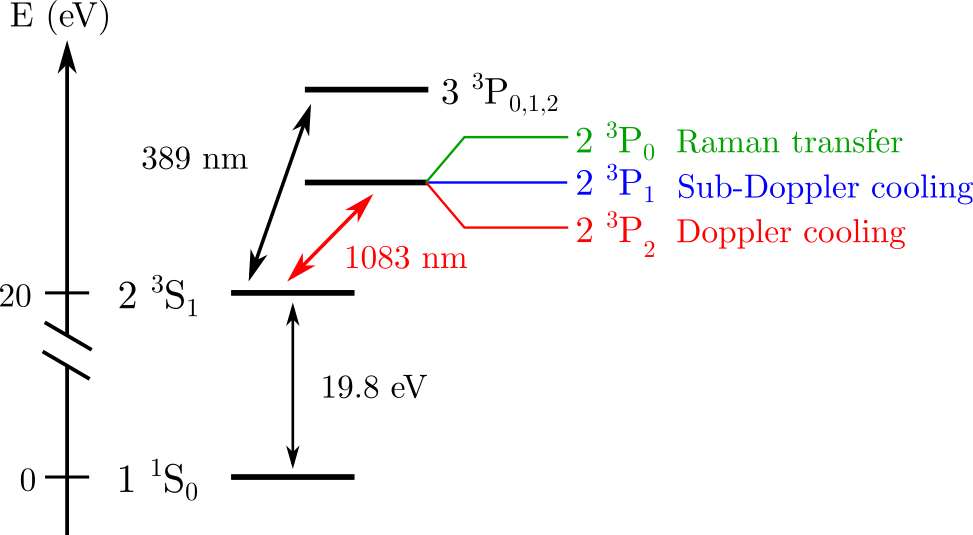
\includegraphics[width=0.9\textwidth]{Fig/Chapter3/niveaux.png}
    \caption{Energy levels of the Helium atom. The metastable state is the triplet state $2 \ ^3S_1$ that we will call the ground state of the metastable Helium atom. Laser cooling is performed on the optical transition $2 \ ^3S_1 \rightarrow 2 \ ^3 P$ of wavelength $\lambda_0 \simeq 1083 \ \mathrm{nm}$. More specifically, we address the transition to  $2 \ ^3 P_2$ or $2 \ ^3 P_1$ depending on the cooling scheme (respectively Doppler and sub-Doppler), as well as the transition to  $2 \ ^3 P_0$ to perform two-photon Raman transfer as we will detail later on.}
    \label{fig:niveaux}
\end{figure}

In the following, we will detail the different experimental steps used to bring a gas of metastable Helium to quantum degeneracy.

%\section{Bose-Einstein Condensation of metastable helium}

\subsection{The source}

To begin the experimental sequence, we first need to excite Helium atoms in the metastable state. As the energy difference between the ground-state and the metastable state is very large, it is impossible to excite the atoms optically. We therefore rather do it through a plasma discharge. The setup is illustrated on Fig.-\ref{fig:source}. The plasma forms between a metallic needle connected to a high voltage power supply ($\sim 2.8 \ \mathrm{kV}$) and the grounded skimmer. The needle is held in a glass tube that is glued to a \textbf{Boron-Nitride (BN)} piece in which a small hole is pierced for atoms to flow through. The piece is inserted into a larger copper piece cryogenically cooled with liquid nitrogen. The role of the Boron-Nitride piece is two fold. First, the good thermal properties of the Boron-Nitride allows the piece to be cooled via the contact with the copper, cooling down in turn the atoms. This is necessary to preliminary reduce the speed of the atoms before laser cooling as we will discuss in the next paragraph. Second, the piece isolates the high voltage needle from the grounded copper to avoid plasma formation in unwanted places.

\begin{figure}
    \centering
    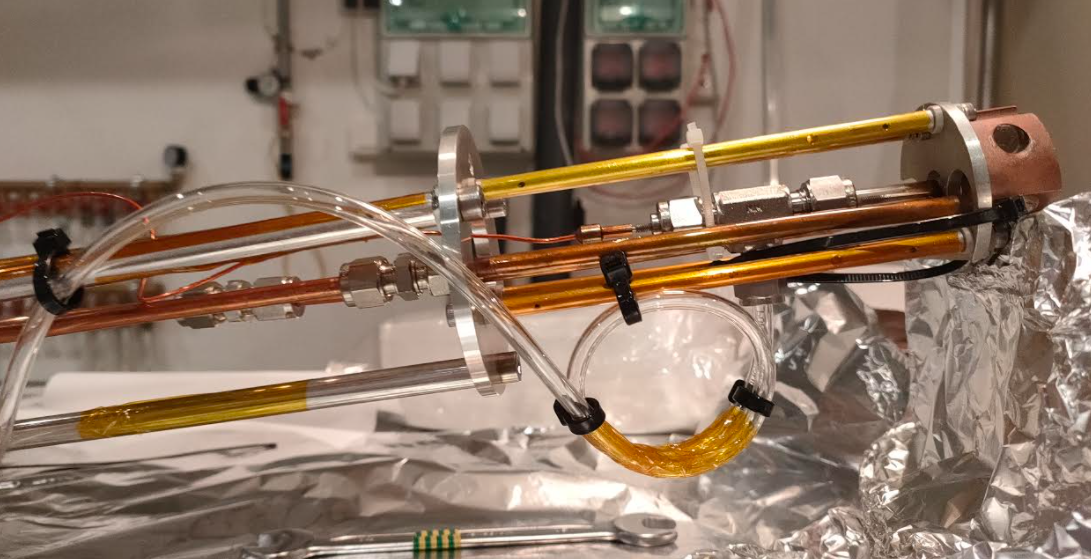
\includegraphics[width=0.9\textwidth]{Fig/Chapter3/source.png}
    \caption{Metastable helium source. (a) Drawing of the source apparatus. Helium atoms (blue arrows) are sent into a glass tube glued into a pierced boron-nitride (BN) piece. A plasma forms between the high voltage needle and the grounded skimmer, exciting the atoms in the metastable state (red arrows). The boron nitride is cooled by thermal contact with a copper (Cu) piece in which liquid nitrogen flows, allowing to significantly reduce the speed of the atoms. (b) Photograph of the source apparatus. The red square illustrates what is represented on the drawing.}
    \label{fig:source}
\end{figure}

The source is a quite sensitive part of the experimental apparatus and was often subject to problems during the span of this thesis. Here are a few things that we learned through the different repairs that need to be checked when troubleshooting the source:

\begin{itemize}
    \item The needle has the tendency to deteriorate over time. When this happens, some metallic particles fall from the needle and end up clogging the small hole in Boron-Nitride, preventing the atoms to flow through. We replaced the needle with a standard metallic cylinder, hoping that it would not deteriorate as fast. While we still could form the plasma without the needle shape, the cylinder still deteriorates, requiring regular operations every few months to unclog the Boron-Nitride piece.
    \item The diameter of the Boron-Nitride piece needs to be very well adapted to the inner diameter of the copper piece to ensure a good thermal contact and to prevent the Boron-Nitride from moving when temperature changes.
    \item The glue holding the glass tube in the Boron-Nitride can contract at low temperatures and add mechanical constraints on the glass tube, sometimes breaking it and causing unwanted atom leakage.
\end{itemize}

We now move on the next experimental step, laser cooling.


\subsection{Laser cooling}

Our experimental cooling sequence uses two types of laser cooling: Doppler and sub-Doppler cooling. Doppler cooling revolves around the absorption of resonant, counter-propagating photons by a two-level atom, reducing its momentum. The absorbed photons are re-emitted spontaneously in a random direction of space, meaning that after a large number of absorption/emission cycles, the variation of momentum induced by spontaneous emission averages out. The only contribution is thus the one of absorption contributing to slow the atom down. This effect is called Doppler cooling as the frequency of the photons seen by the atoms changes with their speed because of the well-known Doppler effect. It is then necessary to account for the Doppler effect to ensure that the photons are resonant with the two-level transition of interest to ensure proper cooling. On the other hand, sub-Doppler cooling designs a variety of cooling techniques revolving around multi-level atomic structures. These techniques allow to reach lower temperatures than Doppler cooling, at the expense of small velocity captures, nevertheless attainable with prior Doppler cooling. 

As shown on Fig.-\ref{fig:niveaux}, we use the $2 \ ^3 S_1 \rightarrow 2 \ ^3 P_2$ transition for Doppler cooling. The state $2 \ ^3 S_1$ has three sub-states $m_J=\{-1,0,+1\}$ whereas the state $2 \ ^3 P_2$ has 5 $m_J=\{-2,-1,0,+1,+2\}$. By using circularly polarised light allowing transitions that increase or decrease $m_J$ by $1$, the transition between these two-states can be equated to an effective two-level transition after a few cycles of absorption/emissions, making it well suited for Doppler cooling. For sub-Doppler cooling, we use the transition  $2 \ ^3 S_1 \rightarrow 2 \ ^3 P_1$ where the excited state also has three sub-states, implementing an effective 3-level lambda structure if the light is properly polarized. The natural line-width of the $2 \ ^3 P$ state is \fcolorbox{red}{white}{$\Gamma = 2 \pi \times 1.6 \ \rm{MHz}$}.

We will not explain here all the details of how laser cooling works, but rather briefly show the main cooling steps of the experimental sequence and give typical experimental numbers. For further details, we refer the reader to previous thesis \cite{hoend2014,bouton_these,cayla_these}.



\subsubsection{Zeeman slower}

As in most cold atoms experiment, the cooling sequence starts with a Zeeman slower. The general idea is to exploit the Zeeman effect with a variating magnetic field to compensate the Doppler shift that reduces as the atoms get slower. This procedure allows to reduce the speed of the atoms of several order of magnitudes, from roughly $1,200 \ \rm{m/s}$ when they exit the source to $50 \ \rm{m/s}$, a speed at which they can be captured in a Magneto-Optical Trap. Note that as helium is very light, our Zeeman slower is quite long compared to other cold atom experiments with a length of $\sim 2.5 \ \rm{m}$. This also explains the need for liquid nitrogen cooling of the source, without which we would need an absurdly long Zeeman slower.

\subsubsection{Magneto-Optical Trap}

While reducing the speed of the atoms is necessary to reach quantum degeneracy, it is also necessary to spatially trap the atoms. This is achieved by combining the radiative pressure force with the magnetic force whose role is to trap the atoms. This is the idea behind the \textbf{Magneto-Optical Trap} (MOT), the cornerstone of every cold atom experiment. A MOT is made of 3 pairs of counter-propagating red-detuned laser beams, one for each direction of space, on which we add a quadrupole magnetic field. In our case, the magnetic field is produced by two coils centered on the $x$-axis in anti-Helmoltz configuration. The current is $16 \ \rm{A}$, resulting in a gradient of $25 \ \mathrm{G/cm}$ at the center of trap.

To load the MOT, we use an intensity of roughly $15 \ \Isat$ per beam and a strong detuning $\delta =-60 \Gamma$ . This serves two purposes: it ensures a large capture velocity, making the loading of the trap efficient, and also keeps the level of light-assisted Penning losses low. We load typically \fcolorbox{red}{white}{$N \simeq 2 \times 10^9$} atoms in $\sim 1.5 \ \mathrm{s}$. In a second time, we look to compress the gas to increase the atomic density by reducing the detuning to $\delta =-12 \Gamma$ . To avoid major Penning losses, we conjointly reduce the total intensity from $90 \ \Isat$ to $0.7 \ \Isat$. This increases the density by a factor 10.

At the end of the MOT phase, we obtain a gas of $N \simeq 2 \times 10^9$ atoms at $T=1.2 \rm{mK}$ of density $n=2.5 \times 10^{10} \ \rm{cm}^{-3}$.

\subsubsection{Red molasses}

The magnetic field is then switched off to go back to regular Doppler cooling. To further cool the atoms, the detuning is significantly reduced to $\delta=-1.5 \Gamma$, while the total intensity is reduced to $0.33 \ \Isat$ to keep the rate of Penning losses constant. The goal is not to reach the lowest possible temperature, but rather to reach a temperature low enough to go under the velocity capture of sub-Doppler cooling effects. After $5 \ \rm{ms}$ of red molasses, we reach $T=120 \ \mu \rm{K}$ with $N\simeq 1.8 \times 10^9$ atoms.

\subsubsection{Grey molasses}

% Grey molasses are a sub-Doppler cooling scheme that works with the so called lambda configuration with two ground states $\ket{g_1}$ and $\ket{g_2}$ and one excited state $\ket{e}$. Through a change of a basis, it is possible to describe the system as a \textbf{dark state}, written as a superposition of $\ket{g_1}$ and $\ket{g_2}$ that does not interact with the light, and bright state. The latter couples to the excited state through dipole transitions driven by the laser light while the former is only accessible through spontaneous emission from the excited state.

Grey molasses are a sub-Doppler cooling scheme that works with the so called lambda configuration with two ground states $\ket{g_1}$ and $\ket{g_2}$ and one excited state $\ket{e}$. Through a change of a basis, it is possible to describe the system as a \textbf{dark state}, written as a superposition of $\ket{g_1}$ and $\ket{g_2}$ that does not interact with the light, and bright state. The grey molasses scheme uses Sisyphus cooling to progressively put more and more atoms into the dark state while cooling them \NOTE{pas ouf} (see \cite{cayla_these,bouton_these} for further details).



The grey molasses stage is implemented with 3 pairs of countra-propagating, blue detuned $\delta =8 \Gamma$ beams with a total power of $28 \ \Isat$. The grey molasses stage lasts $5 \mathrm{ms}$ after which we obtain $N \simeq 1.7 \times 10^9$ atoms at $T \simeq 15 \ \mu K$. While this temperature is already quite low, the cooling steps we have described so far are not enough to reach the kinds of temperatures and densities required to reach quantum degeneracy. We thus need another non-optical cooling technique for the last steps of the experiment.

\begin{figure}
    \centering
    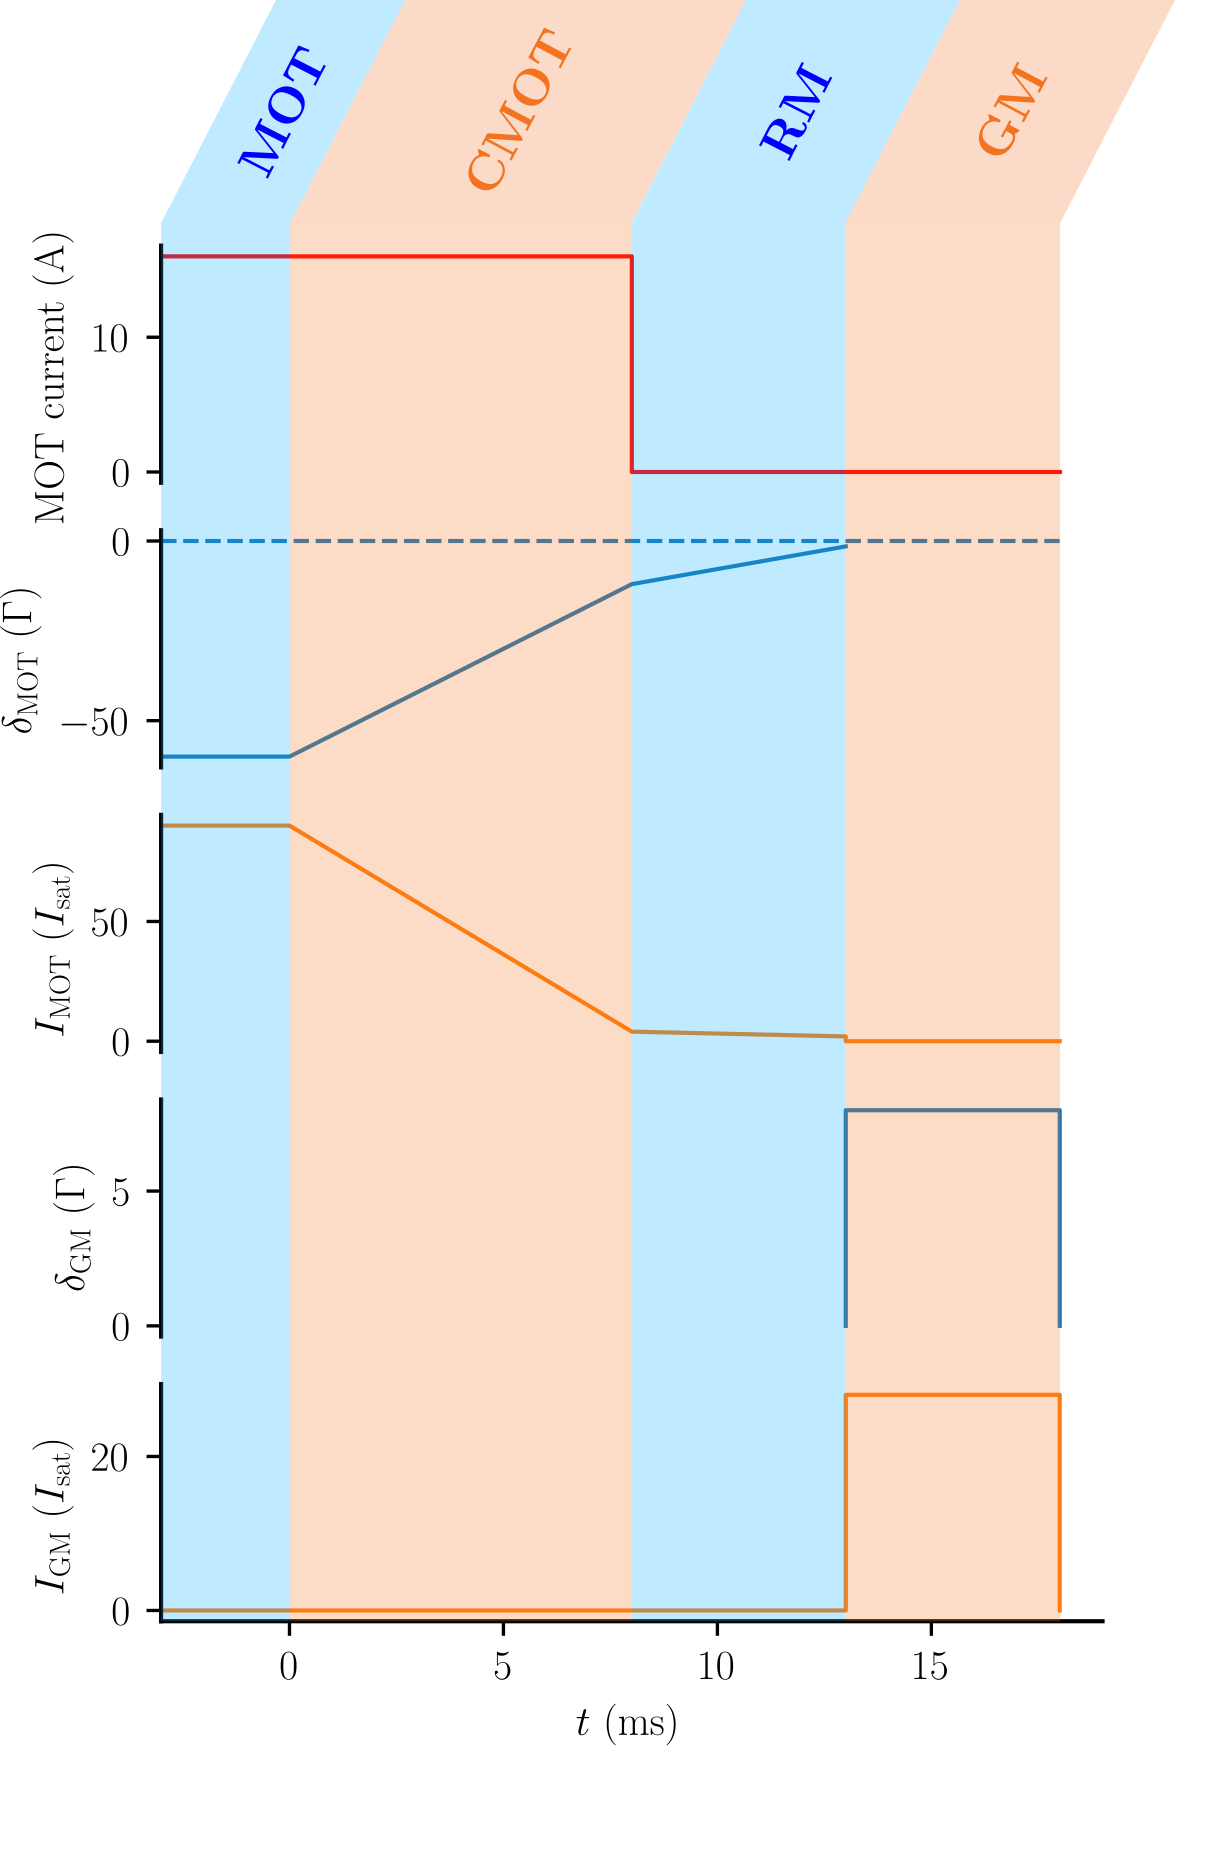
\includegraphics[width=0.7\textwidth]{Fig/Chapter3/laser_cooling.png}
    \caption{Laser cooling sequence. The time $t=0$ corresponds to the beginning of the compressed MOT step, preceded by the MOT step that lasts $1.5 \ \rm{s}$. The initials RM and GM corresponds to Red Molasses and Grey Molasses respectively. Current values are represented in red, light frequencies in blue and light intensities in orange.}
    \label{fig:my_label}
\end{figure}

\subsection{Evaporative cooling}

Evaporative cooling was derived from the simple idea that if one is able to selectively remove the hottest particles of an ensemble, the remaining ones will thermalize at a lower temperature. This is exactly what we do when we blow on a cup of coffee, removing the hottest coffee molecules vaporized above the surface to cool down the entire cup of coffee. Evaporative cooling therefore requires to find a way to remove only the hottest atoms while ensuring that the collision rate amongst the remaining atoms is high enough for a proper thermalization. 

There are two main ways to implement evaporative cooling depending on the kind of trap from which we will remove the atoms. The historical one is called \textbf{radio-frequency (RF) evaporation} and is performed with magnetic traps. Let us illustrate it with the example of atoms with 3 magnetic sub-states, $m_J=\{-1,0,1\}$. If we put these atoms inside a quadrupole magnetic field forming a magnetic gradient, we find that one of the sub-states is trapped, let us say $m_J=1$, the sub-state $m_J=0$ does no interact with the magnetic field and is therefore not trapped, just like the sub-state $m_J=-1$ which is anti-trapped. Because of the Zeeman effect, the energy difference between the different sub-states depends on the value of the magnetic field and therefore on the position of the atoms in the trap. The hottest atoms are the ones with the larger kinetic energy and that therefore reach positions farther away from the center of the trap. The idea is then to use a radio-frequency wave to drive the transition between the trapped and non-trapped sub-states and carefully choose its frequency so that the process is resonant only for the regions farther from the center of the trap, effectively removing the hottest atoms. The frequency of the RF wave is then progressively reduced to be more and more selective on the energy for which atoms are removed, thus progressively cooling down the gas. An important point is that the frequency must be ramped down slow enough for the gas to have enough time to thermalize. The duration of RF evaporation is thus inherently limited by the collisions properties of the gas, and therefore its density.

The second way to implement evaporative cooling is \textbf{optical evaporation} used in optical traps. With high intensity, far-detuned laser beams, the electric field is strong enough to induce a dipole moment in the atom, causing them to be attracted to the maximum intensity of the field, effectively trapping them. The depth of the trap is then set by the intensity of the laser light. In this case, evaporation is quite simple: decreasing the intensity decreases the depth of the trap, allowing atoms with a high kinetic energy to escape the trap. Evaporation is then performed by ramping down the intensity of the laser light. Interestingly, optical traps allow to reach higher trapping frequencies than magnetic trap, resulting in higher densities and thus better collision rates, meaning that evaporation can be done much faster.

For our experimental purpose, we need to devise what kind of trap to use. An optical trap would first seem to be the obvious answer as evaporation can be done way quicker, reducing the experimental cycle time and thus making data taking more efficient. The problem however with optical traps is that their capture volume is quite small and efficient loading would be hard to achieve with the kind of gas we obtain after laser cooling. We thus opted for an hybrid configuration where the atoms are first loaded in a magnetic quadrupole trap where a first evaporation stage is performed up to temperatures for which they can be efficiently loaded in a optical trap in which we perform a final evaporation stage to reach Bose-Einstein condensation.

\subsubsection{Magnetic trap}

Before loading, the atomic gas is optically pumped into the trapped state $m_J=1$. To do so, we create a bias field oriented along the $z$-axis to set the quantification axis and shine $\sigma_{+}$ resonant polarized light unto the atoms for $700 \ \mu \rm{s}$. We then create a magnetic quadrupole field with the same coils used for the MOT to produce an initial gradient of $\sim 5 \ \rm{G/cm}$ and load $N \simeq 1.7 \times 10^{9}$ atoms into the trap. Note that because of spin conservation laws, the Penning collision rate is highly reduced for a spin-polarized gas as mentioned in the beginning of this chapter. We therefore safely go to higher densities by compressing the trap, increasing the gradient to $\sim 35 \ \rm{G/cm}$. The evaporation cooling is performed in $3 \ \rm{s}$, reducing the number of atoms to a typical $N=100 \times 10^6$. The final temperature is $T \simeq 70 \mu K$. Note that while this is higher than what we had at the end of laser cooling as the gas is heated up when loaded in the magnetic trap, we have significantly increased the density and therefore got closer to quantum degeneracy.

\subsubsection{Crossed Optical Dipole trap}

The Optical Dipole Trap (ODT) is made with two crossing far detuned 1550nm laser beams whose intensity is stabilized with PID locking. We label these two beams ODT1 and ODT2, the second beam being obtained from the first one in a butterfly-like shape (see Fig.-\ref{fig:scheme_odt_lattice}). Their respective waists are $133 \ \mu \rm{m}$ and $63 \ \mu \rm{m}$ and the maximum power for ODT1 is $18 \ \rm{W}$. The ODT is loaded by ramping up the laser power while ramping down the current in the quadrupole coils. The overlap between the two traps is finely adjusted thanks to magnetic biases fields. As the ODT is very narrow, we typically only load $N \simeq 5 \times 10^6$ but reduce the temperature by a factor 2 while increasing the density by two orders of magnitude. The final evaporation stage is done by ramping down the laser power in $400 \ \rm{ms}$. We adapt the final laser power to chose the number of atoms in the BEC, from a few thousands to roughly $N \simeq 10^6$ at maximum. The trapping frequencies depend from the chosen final power with typical values $2\pi \times (\omega_x,\omega_y,\omega_z)= (81,352,320) \ \rm{Hz}$ for $\NBEC \simeq 6 \times 10^5$ and $2\pi \times (\omega_x,\omega_y,\omega_z)= (41,173,180) \ \rm{Hz}$ for $\NBEC \simeq 5 \times 10^3$ as we wish to use for the \kmk correlations measurements.


\begin{figure}
    \centering
    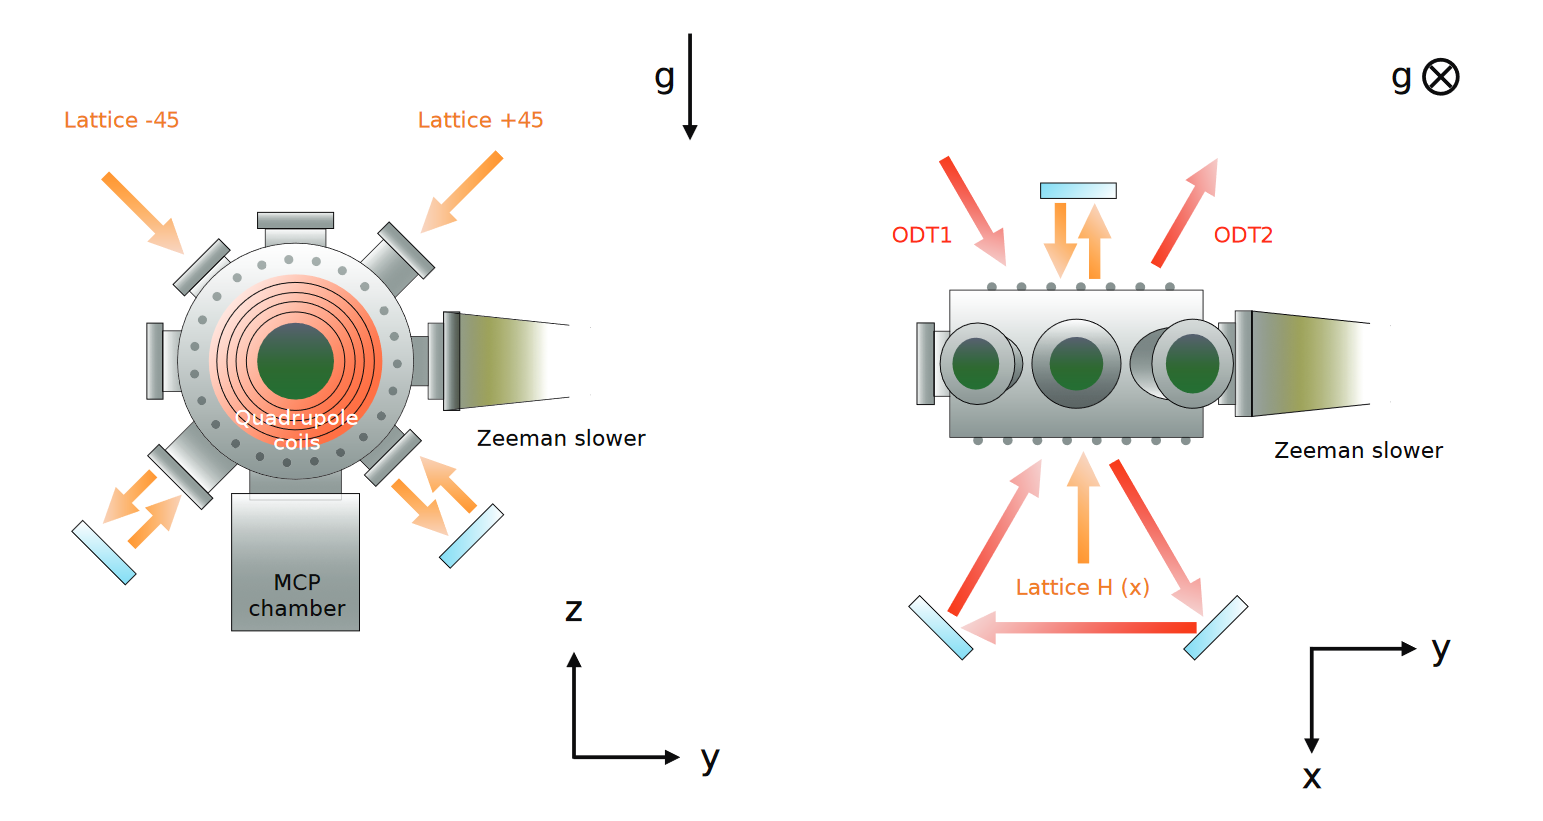
\includegraphics[width=\textwidth]{Fig/Chapter3/scheme_odt_lattice.png}
    \caption{Orientation of the ODT and lattice beams in the experiment. Taken from \cite{cayla_these}.}
    \label{fig:scheme_odt_lattice}
\end{figure}

\begin{figure}
    \centering
    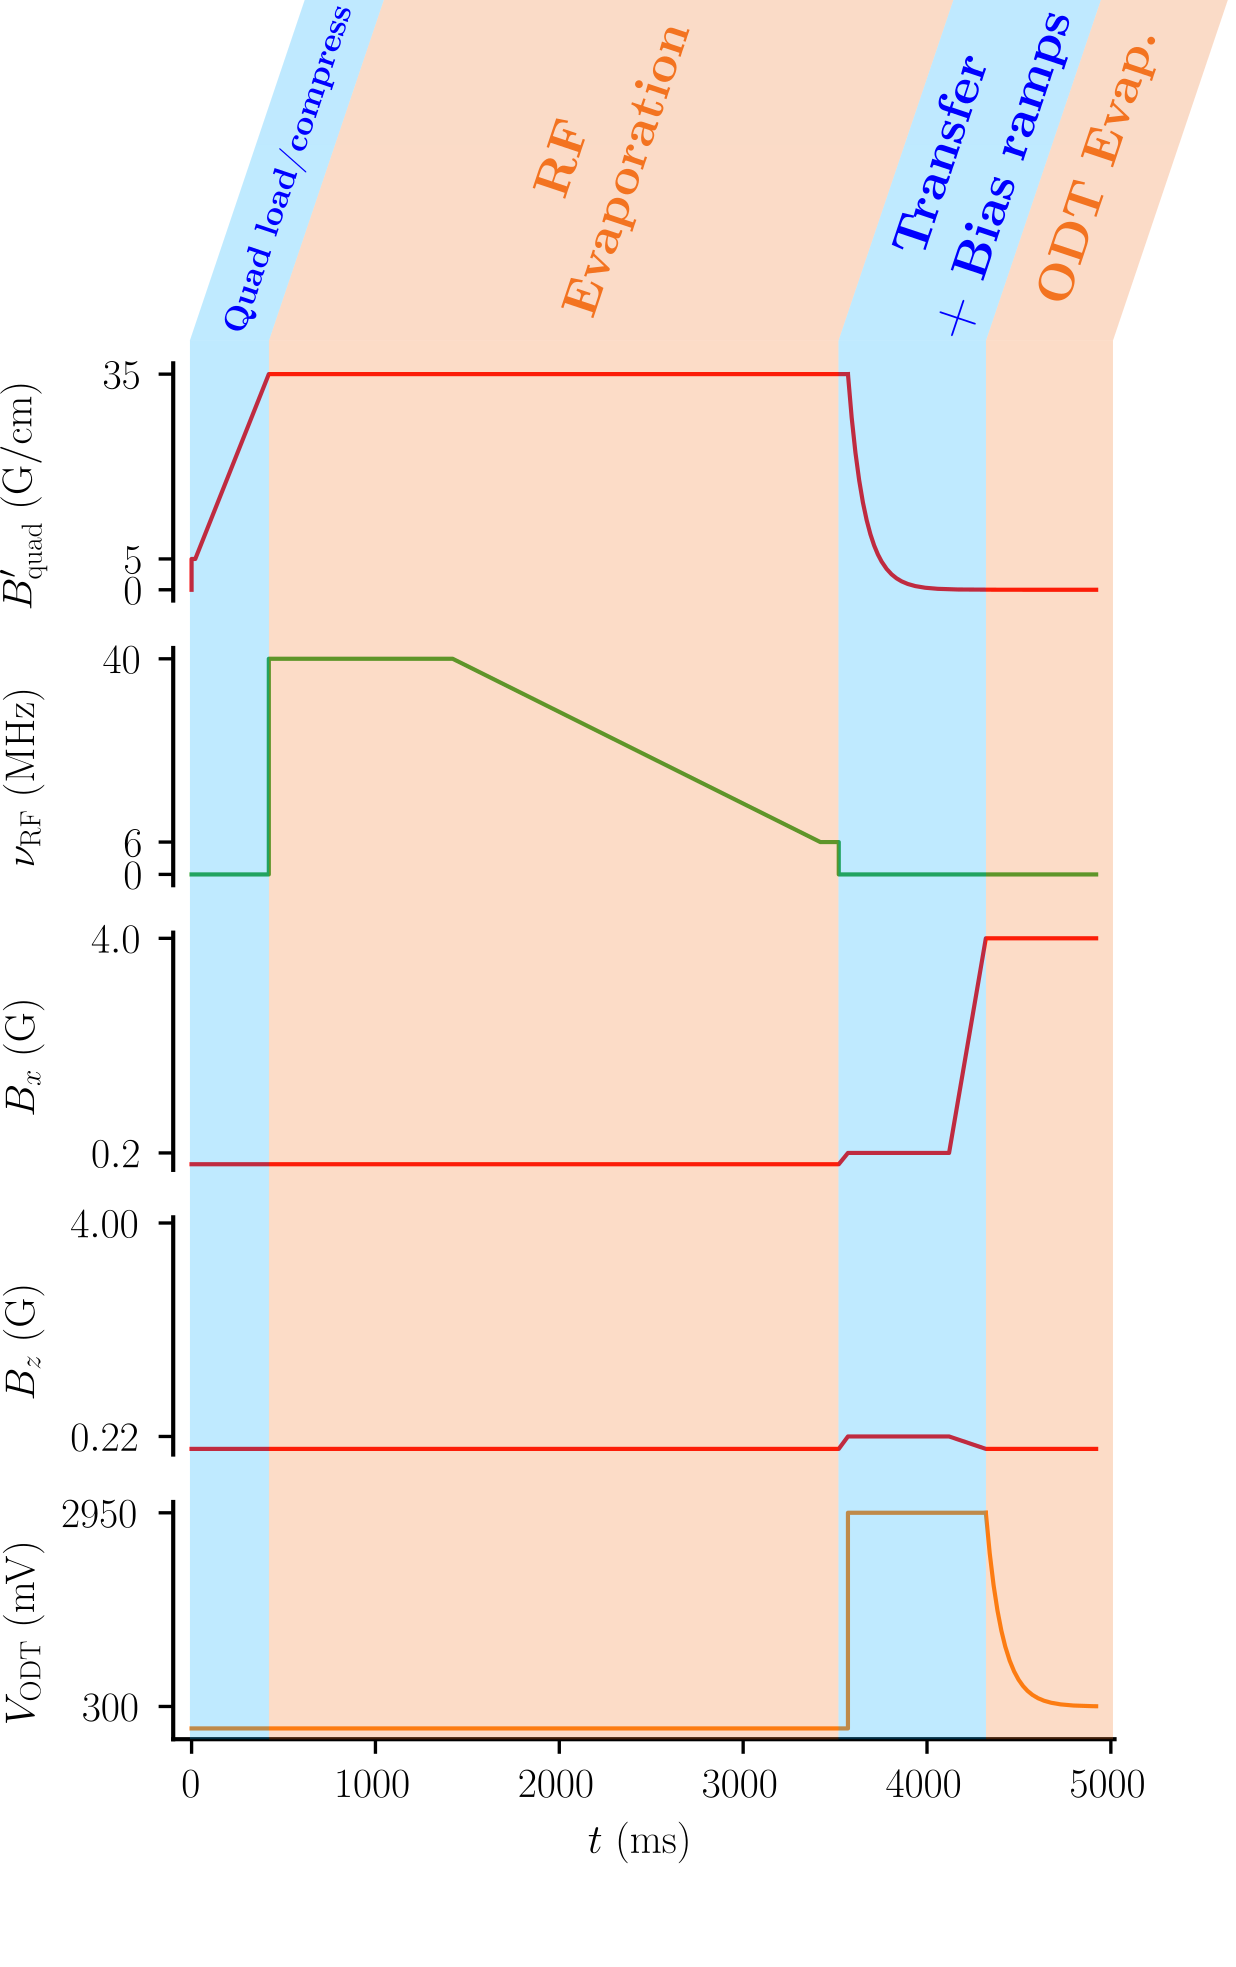
\includegraphics[width=0.7\textwidth]{Fig/Chapter3/condensation_sequence.png}
    \caption{Condensation sequence. The red lines correspond to magnetic fields, \ie the quadrupole trap gradient and the $x$ and $z$ biases (no bias along $y$ is used), the green line to the frequency of the RF wave used to peform the evaporation and the orange line to the ODT power, here expressed in terms of photodiode voltage $V_{\rm{ODT}}$.}
    \label{fig:my_label}
\end{figure}

\subsection{Optical imaging}

While the specificity of our experiment is its electronic detection technique, we also use more classical optical imaging techniques that are way more convenient to observe and characterize the gas at the different steps of the experimental sequence.

\subsubsection{Fluorescence imaging}

The first kind of optical imaging technique that we use is fluorescence imaging. After a time of flight of a few ms to access the momentum space, we shine for $100 \ \mu \rm{s}$ with the MOT beams resonant light on the atoms that absorbs the photons and re-emits them spontaneously in all directions of space. These photons can be detected with an InGaAs camera located on top of the science chamber with its optical axis oriented along the vertical $z$ direction. Fluorescence imaging is mainly used to characterize all steps prior to the loading in the optical trap after which the gas becomes too small for the resolution of the camera.
 
\subsubsection{Absorption imaging}

To image the atoms in the ODT or the BEC itself, we use absorption imaging. We shine a probe beam of weak intensity on resonance with the $2 \ ^3 S_1 \rightarrow 2 \ ^3 P_2$ transition unto the atomic cloud and observe its ``shadow'' with a second InGaAs camera. The intensity of the detected light depends directly on the quantity of light absorbed by the atoms and therefore the density of the cloud. The camera is located on the side of the science chamber and its optical axis forms a small angle with the horizontal direction.

While the resolution of the camera of $12 \ \mu \rm{m}$ in the image plane is not suited to make in-situ images, the BEC can be properly observed after a small time-of-flight of a few ms. Interestingly, we can obtain from the absorption images the number of atoms in the BEC $\NBEC$ by measuring the Thomas-Fermi radius of the gas after a small TOF \cite{bouton_these}.



\subsection{3D optical lattice}

We now continue the description of our experimental apparatus with one of the key ingredients of the physics we want to study, the 3D optical lattice. Its main characteristics are: 

\begin{itemize}
    \item The 3D lattice is made from a single narrow linewidth laser capable of delivering up to $15 \ \mathrm{W}$. Its wavelength is $1550 \ \rm{nm}$, \ie far from any atomic resonance just as for the Optice Dipole Trap, so that the atoms are trapped at the maximum values of intensity.
    \item  The main beam is divided into 3 independent beams, one for each direction of space, that are sent on the science chamber to make the optical lattice as illustrated on Fig.-\ref{fig:scheme_odt_lattice}. One of the beam is horizontal (named H) and perpendicular to the axis defined by the Zeeman slower, will the other two form a $\pm 45^{\circ}$ angle with horizontal, hence their name, +45 and -45.
    \item  Each beam is retro-reflected to create the interferences necessary for the lattice pattern, but detuned by $20 \ \rm{MHz}$ from the other directions so they do not interfere with one another.
    \item In this configuration, the lattice spacing $d$, \ie the distance between two lattice sites is $d=\lambda/2 = 775 \ \rm{nm}$.
    
    % From this we define the recoil momentum and the associated recoil energy:
    
    % \begin{equation}
    %     k_d = \frac{2 \pi}{d}, \ E_r = \frac{\hbar^2 k_d^2}{2 m}
    % \end{equation}
    
    % \noindent In the following, we will often use $k_d$ as the momentum unit and $E_r$ as the unit for the lattice depth unit with $V_0 =  s E_r$.
    
    \item A fraction of the power of each beam is sent on a photodiode whose signal is used for the feedback loop of a PID controller used to lock the power on the desired value.
    
    \item Because of the Gaussian shape of the beam, the atoms feel the same external trapping frequency $\omega_{\rm{trap}} = 2 \pi \times 140 \times \sqrt{s}$ in the three directions of space.  
    
\end{itemize}



 
\subsection{Calibration of the lattice depth}

As we have seen in Chapter \ref{sec:chapter_2}, the depth of the lattice potential and hence the ratio $U/J$ is a crucial parameter that determines the phase of the lattice gas. It is then necessary to precisely calibrate this value prior to any experiment. The idea of the calibration is to associate a given value of the lattice depth $s$ to a command voltage for the PID controller. As the power of each of the three beams are independent, the calibration must be done for each of the three beams alike. 

\begin{figure}
    \centering
    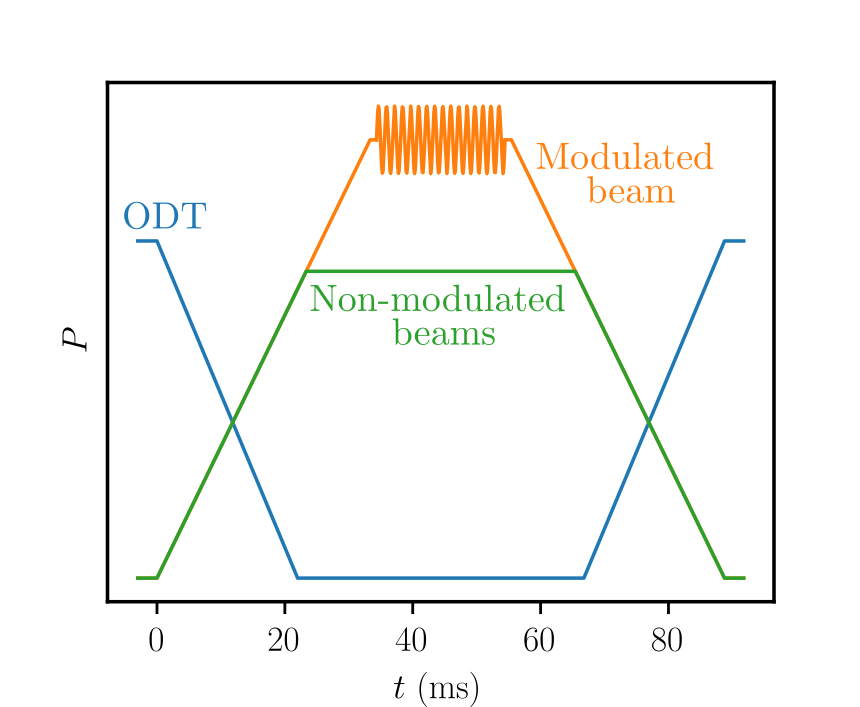
\includegraphics[width=0.7\textwidth]{Fig/Chapter3/lattice_modulation.png}
    \caption{Calibration of the lattice amplitude. The atoms are loaded in the lattice by ramping down the ODT power (red) and ramping up the lattice power (blue). The beam to calibrate is then modulated while the two other beams are set to be $30 \%$ to avoid excitations in directions different from the one that is being calibrated. Finally, the atoms are loaded back in the ODT to measure the number of remaining atoms with absorption imaging.}
    \label{fig:calib_process}
\end{figure}

To do so, we modulate the amplitude of one of the lattice beam at frequency $f_{\rm{mod}}$ for a duration $t_{\rm{mod} }= 20 \ \rm{ms}$, adding two sidebands in the lattice light spectrum $f \pm f_{\rm{mod}}$. When $2 f_{\rm{mod}}$ is close to the resonance frequency $f_{\text {res }}=\left(E_{2}(q=0)-E_{0}(q=0)\right)/\hbar$, it is possible to excite the atoms in the lowest energy band to the second excited band with a resonant two-photon process. As $f_{\text {res }}$ is dependent from the lattice depth, the idea is to scan the value of $f_{\rm{mod}}$ to find the resonance from which we deduce the value of the lattice depth. If the amplitude of the lattice at which we perform the calibration is not too high (we use $s= 10$ in practice), atom in the second excited band are not trapped and therefore lost. When we are perfectly at resonance, most atoms should then be lost, an effect that we can observe via absorption imaging. To make things more convenient, we load back the atoms into the ODT (see Fig.-\ref{fig:calib_process}) before taking the absorption image to avoid the diffraction induced by the lattice beams and properly count the atoms. We therefore measure the number of remaining atoms in the BEC after this procedure as a function of $f_{\rm{mod}}$ and fit the data to find the minimum and so $f_{\rm{res}}$ as illustrated on Fig.-\ref{fig:lattice_calibration}. By calculating the energy bands, we obtain the relation between the lattice depth and the value of $f_{\rm{res}}$ that allows us to finally obtain the value of the lattice depth. We repeat this procedure for each lattice beams, where the power of the two non-modulated beams are lowered by $30 \%$ so that the cloud is not excited in the other directions.

\begin{figure}
    \centering
    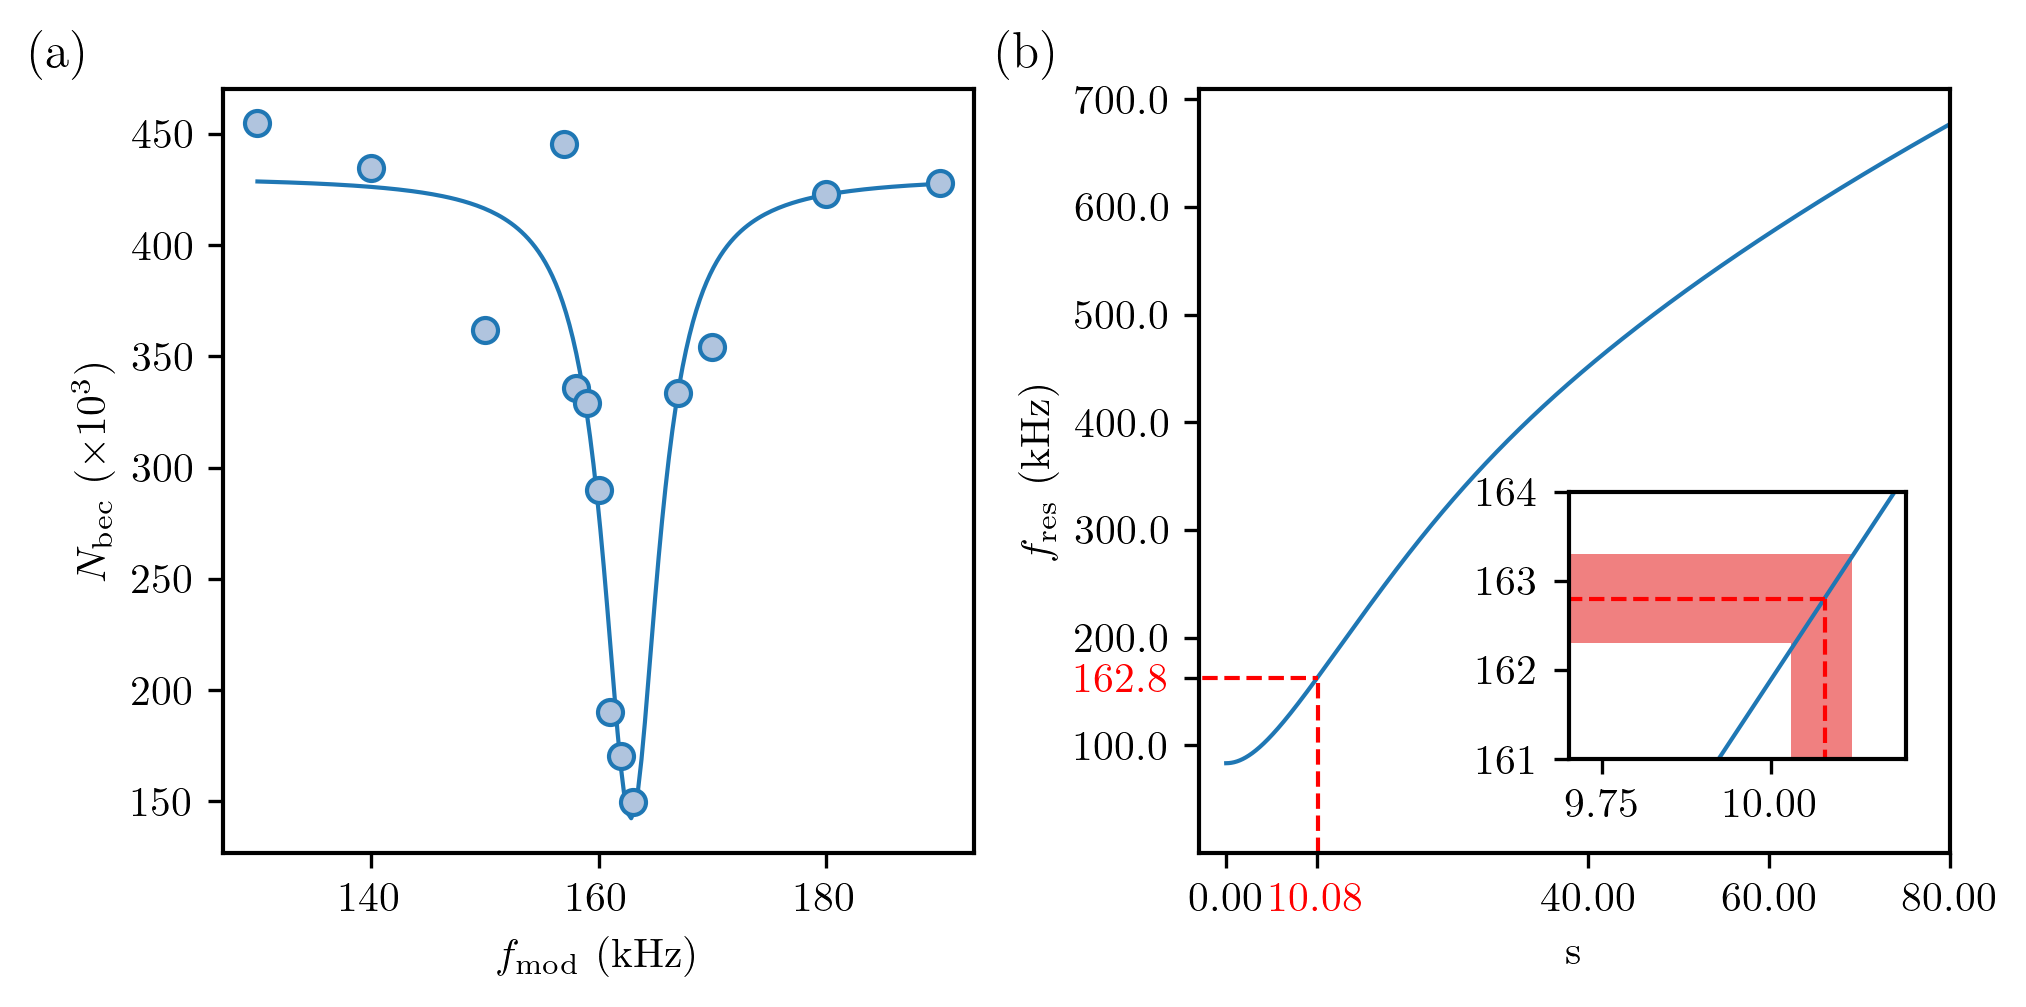
\includegraphics[width=\textwidth]{Fig/Chapter3/lattice_calibration.png}
    \caption{Calibration of the lattice depth. (a) Variation of the atom number after the calibration procedure as a function of the modulation frequency $f_{\rm{mod}}$. A clear resonance of frequency $f_{\rm{res}}=162.8 \ \rm{kHz}$ is observed. (b) Plot of the resonance frequency $f_{\rm{res}}$ as a function of the lattice depth $s$. The red dashed lines illustrates how the lattice depth is obtained from the measurement of $f_{\rm{res}}$ on the left panel.}
    \label{fig:lattice_calibration}
\end{figure}


\section{Metastable Helium detection}

%\subsection{Electronic detection}

Contrary to most cold atoms experiments that rely exclusively on optical detection techniques, our experiment revolves around a \textbf{single-atom resolved} \textbf{electronic} detection technique of which we will present the main features in this section. For a more thorough and technical description of the $\He$ detector, we refer the reader to the manuscript of Hugo Cayla \cite{cayla_these}.

\subsection{Micro-Channel Plates}

The first main element of the $\He$ detector is the \textbf{Micro-Channel Plate} (MCP). A Micro-Channel Plate is essentially a piece of metal in which an array of small holes, the micro channels, have been drilled. If a particle falls into one of the channels and hits its walls, it can extract one electron from the metal provided that the particle is energetic enough ($\sim$ a few eV). While MCPs cannot be used in most cold atoms experiment as the atoms are not energetic enough to extract this first electron, they are suited to detect $\He$ thanks to the high energy of the metastable state. An electric field is applied so that the electron is accelerated downwards and subsequently hits the walls of the channel to extract additional electrons, that will also extract more electrons and so on, just like an avalanche process. The MCP then works to amplify the initial discharge into a shower of a large number of electrons that can be properly detected. 

Practically speaking, we use two MCPs in a z-stack configuration forming a herringbone pattern (see Fig.-\ref{fig:MCP}) to ensure the continuity of the electron shower. They are polarized with a voltage of $2.4 \ \rm{kV}$. Using two plates is necessary to obtain a high enough amplification factor of $10^4$. The channels are drilled with a $20^{\circ}$ degree angle from the surface of the MCP in order to avoid that the atoms fall right through the channels without hitting the walls. Another important characteristics of the MCP is the \textbf{open-to-air ratio}, \ie the ratio between the holes surface and the total surface of the MCP. This must be as high as possible to avoid that atoms hit the MCP but not in a channel, thus losing the first electron. The new generation of MCPs we are using for the experiments conducted in this thesis (Hamamastu F9142-01 MOD6) implements a technology improving the open-to-air ratio to $90\%$ for the top plate and $70 \%$ for the bottom one.

\begin{figure}
    \centering
    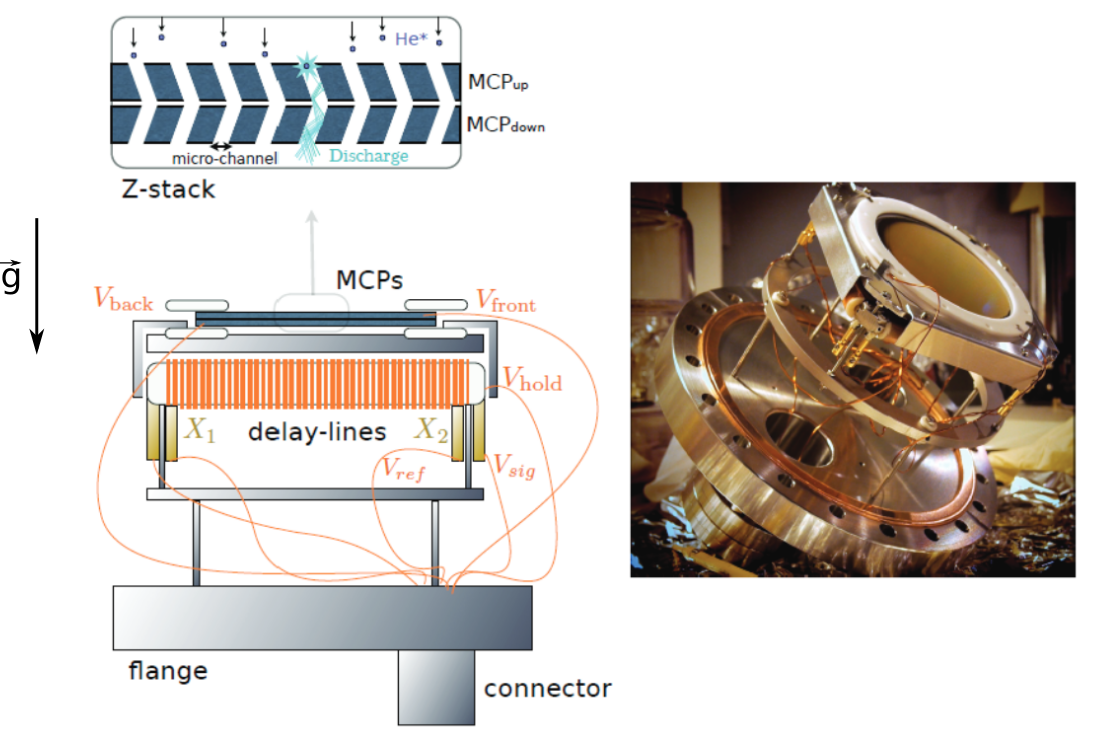
\includegraphics[width=0.9\textwidth]{Fig/Chapter3/MCP.png}
    \caption{$\He$ detector. The top left schematic illustrates how the MCP works, while the bottom left schematic shows the entirety of the $\He$ detector with the delay-lines located underneath the two stacked MCPs. The right image is a photograph of the apparatus. Taken from \cite{cayla_these}.}
    \label{fig:MCP}
\end{figure}



The MCPs by themselves would be useless as we need something to detect the electron shower to know where a given atom has fallen. In high-energy particle physics experiments in which MCPs are the most widely used, this is done by putting behind the MCPs a phosphorus screen or photo-multipliers which are however not suited to our needs as they only record a 2D information. To measure the 3D momentum of the atom, we need to know the time of arrival of the atom in addition to the $x$ and $y$ coordinates at which it fell on the MCP. To this end, we use what we call \textbf{delay lines}.

\subsection{Delay lines}

\label{sec:delay_lines}

The delay lines consists of two metallic wires of length $L_{x,y}=20 \ \rm{m}$ wrapped around a hundred times around a holding board located beneath the MCPs. The electronic shower created by the MCPs couples into the delay lines, creating an electronic pulse that propagates at speed $v_g=10^6 \ \rm{m/s}$ in the two directions of each delay lines as illustrated on Fig.-\ref{fig:delay_lines}. By recording the times of arrivals at each ends of the delay lines labelled $t_{x_1},t_{x_2},t_{y_1}$ and $t_{y_2}$, we reconstruct the coordinates and time of impact with:


\begin{equation}
    x_{\rm{det}}=\frac{1}{2} (t_{x_1}-t_{x_2})v_g
\end{equation}
\begin{equation}
    y_{\rm{det}}=\frac{1}{2} (t_{y_1}-t_{y_2})v_g
\end{equation}
\begin{equation}
    t_{\rm{det}}=t_{x_{1}}+t_{x_{2}}-\frac{L_{x}}{v_{g}}=t_{y_{1}}+t_{y_{2}}-\frac{L_{y}}{v_{g}}
    \label{eq:tdet_MCP}
\end{equation}

\begin{figure}[ht!]
    \centering
    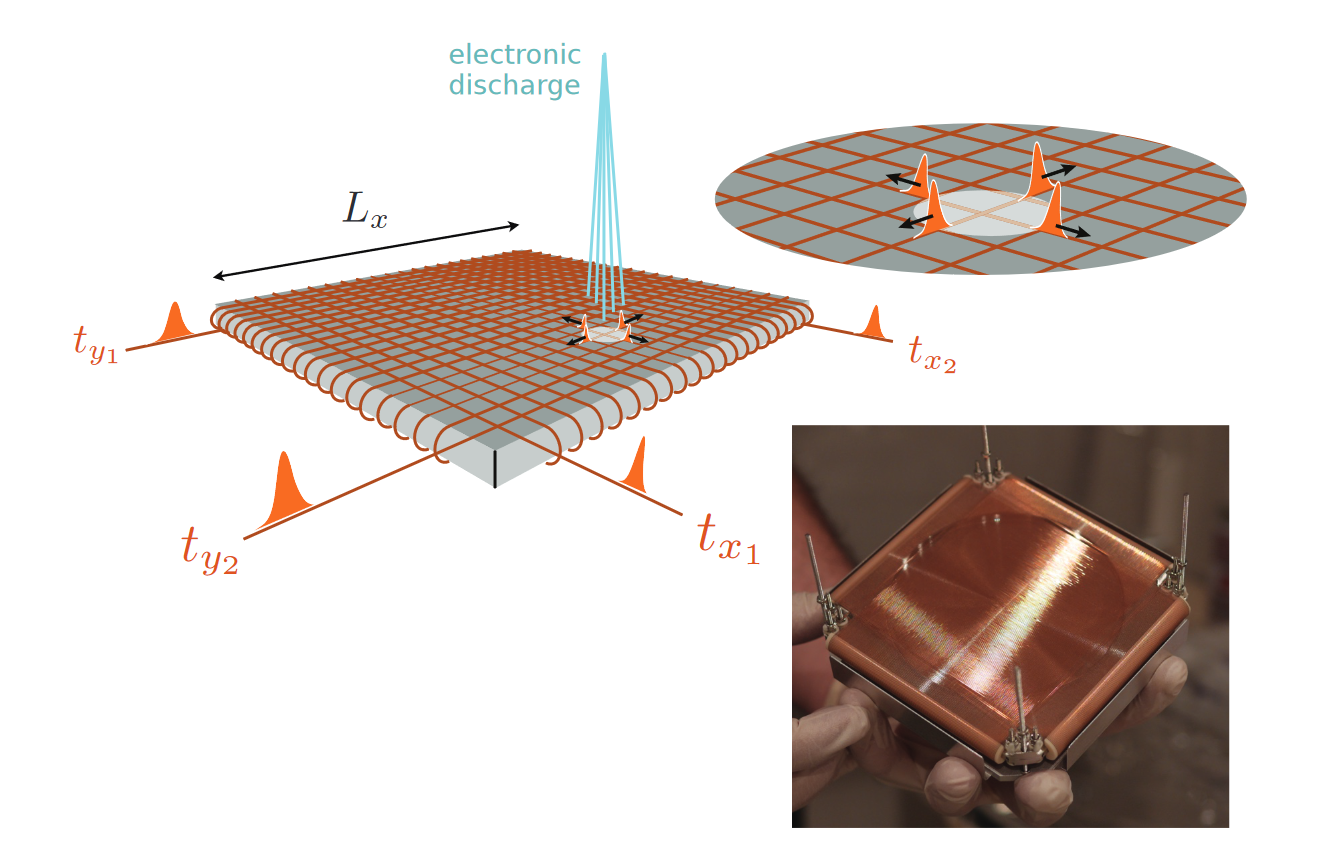
\includegraphics[width=\textwidth]{Fig/Chapter3/delay_lines.png}
    \caption{Schematic of the delay lines. The electronic discharge couples to the delay lines and propagates in the two directions of the delay lines. The times of arrival are recorded at each ends of the delay lines.}
    \label{fig:delay_lines}
\end{figure}

We now need to understand how to use the values of $x_{\rm{det}}$, $y_{\rm{det}}$ and $t_{\rm{det}}$ to obtain the 3D momentum $\bm{k}$ of the detected atoms. As detailled in Chapter \ref{sec:chapter_2}, when there are no interactions between the atoms, the density after a TOF $t_{\rm{TOF}}$ $\rho_{\rm{TOF}} (\bm{r},t_{\rm{TOF}})$ maps the in-trap momentum distribution with the simple ballistic relation $\hbar \bm{k} = m \bm{r}/t_{\rm{det}}$ provided that the TOF is long enough to access the far-field regime. 

To verify this condition, the MCPs are located at a distance $D_{\rm{MCP}}=43 \ \rm{cm}$ below the atom trap, corresponding to a TOF $t_{\rm{TOF}}=297 \ \rm{ms}$ for atoms with a zero vertical momentum to reach the detector. We remind that the far-field condition writes (see equation \ref{eq:far_field}):

\begin{equation}
    t_{\rm{FF}} = \frac{mL^2}{2 \hbar} \simeq 25 \ \rm{ms} \ll t_{\rm{TOF}}
\end{equation}

\noindent meaning that we are deep into the far-field regime. Note that this condition is made easier to fulfill thanks to the small mass of the Helium atom. 

For now, we will assume that there are indeed no interactions during the TOF so that the ballistic relation is true. This hypothesis will be verified in the next sections. We thus need to know how to determine the position vector $\bm{r}$ where the atom is detected after the TOF. While $x$ and $y$ are obtained directly from $x_{\rm{det}}$ and $y_{\rm{det}}$, it is not so clear how to obtain $z$ from what we measure with the delay lines.


When the trapping potential is turned off, the atoms experience a free fall under the sole effect of gravity. The vertical position $z$ of an atom with an initial speed $v_z$ after a time $t$ is, taking the origin of the reference-frame at the center of the MCP and $t=0$ when the trap is turned off:

\begin{equation}
    z(t)= \frac{1}{2} gt^2 + v_z t -  D_{\rm{MCP}}
\end{equation}

% \noindent with $D_{\rm{MCP}}=43 \ \rm{cm}$ the vertical distance between the MCPs and the center of the trap. We define $t_{\rm{TOF}}$ the time necessary for atoms with $v_z=0$ to reach the detector. In the experiment, this time is $t_{\rm{TOF}}=297 \ \rm{ms}$. From this we write:

\noindent As $t_{\rm{TOF}}$ the time necessary for atoms with $v_z=0$ to reach the detector, we can write:

\begin{equation}
    D_{\rm{MCP}} = \frac{1}{2} g t_{\rm{TOF}}^2
\end{equation}

\noindent to obtain

\begin{equation}
     z(t)= \frac{1}{2} g(t^2-t_{\rm{TOF}}^2) + v_z t
\end{equation}


\noindent Finally, the time at which an atom is detected on the detector at $z=0$, which is the quantity we experimentally measure, verifies:

\begin{equation}
    \frac{1}{2} g(t_{\rm{TOF}}^2-t_{\rm{det}}^2) = v_z t_{\rm{det}}
\end{equation}

\noindent To use the convenient ballistic relation $\hbar \bm{k} = m \bm{r}/t_{\rm{det}}$, we then define $z$ so that $z=\frac{1}{2} g(t_{\rm{TOF}}^2-t_{\rm{det}}^2)$.

\subsection{Detection of the electronic pulses and resolution of the detector}

As we have seen in the last paragraph, the precision with which we measure the momentum of the atoms depends directly on the precision with which we measure the arrival times $(t_{x_1},t_{x_2},t_{y_1},t_{y_2})$. It therefore crucial to devise a procedure to attribute to a pulse an arrival time as precisely and reliably as possible. The main difficulty comes from the fact that the amplitude of the pulses varies as the different electronic showers do not couple with the same efficiency in the delay lines. If we were to attribute the arrival time by identifying when the signal goes above a given threshold voltage, a high amplitude pulse would be detected sooner than a low amplitude one. To circumvent this issue, we use a \textbf{constant fraction discriminator} (CFD) that produces the following signal:

\begin{equation}
    V_{\rm{CFD}}(t)=V_{\text {pulse }}(t)-f_{c} \times V_{\text {pulse }}(t)\left(t-\tau\right)
\end{equation}

\noindent where $f_c \in [0,1]$ and $\tau$ a delay. The resulting signal is therefore a bimodal pulse that crosses zero, setting the reference to trigger a 0-1V with sharp raising edge signal that is then fed to a FPGA-based Time to Digital Converter (TDC) to convert it to a digital time. The TDC coding step is $t_0 = 120 \ \rm{ps}$ defining an in-plane pixel of size:

\begin{equation}
    x_0 = y_0 = \frac{1}{2} t_0 v_g = 60 \ \mu \rm{m}
\end{equation}

 \noindent This is the theoretical best resolution that we can obtain with these electronics corresponding to a momentum resolution $\sigma = 1.4 \times 10^{-3} k_d$. In practice, the resolution is not as good, whether it be because of the noise of the electronics are any experimental defect that we might overlook.
 
 To experimentally measure the resolution of the detector, we can make use of the Hanbury Brown and Twiss effect. As explained in Chapter \ref{sec:chapter_1}, we expect to observe for a system with Gaussian statistics that the second-order correlation function goes to 2, $g^{(2)} (\bm{k},\bm{k})=2$, and decays on a typical scale $1/L$, $L$ being the spatial size of the system. If however the width of the correlation function is not much larger than the resolution of the detector, the second-order correlation function is broadened and the amplitude reduced. One can then create a large system so that the second-order correlation function is narrow enough so that the resolution of the detector affects it, and deduce the value of the resolution from the observed reduction of the amplitude.
 
 This method was applied in Hugo Cayla's thesis \cite{cayla_these} with Mott insulator gas of $40 \times 10^3$ atoms to measure that the resolution of the detector is isotropic and equal to \fcolorbox{red}{white}{$\sigma_{\rm{MCP}} = 2.5(1) \times 10^{-3} \ k_d$}. However, in this case, the effect of the resolution is not very strong as the spatial size of the gas is not very larger. We then tried to complement these measurements by using thermal gases of $\sim 200 \times 10^3$ atoms produced in the ODT, taking advantage of the anistropy of the trap so that the gas is large in the direction where the trapping frequency is small. In this direction, the correlation function is then expected to be very narrow and thus heavily affected by the resolution of the detector. We were indeed able to observe that the amplitude of the second-order correlation function is reduced up to 1.33(1) from which we deduced \fcolorbox{red}{white}{$\sigma_{\rm{MCP}} = 2.9(3) \times 10^{-3} \ k_d$} which is in fact quite consistent with the previous measurement. We note at this point that the correlation function measurements that we shall present in the next chapter are conducted with relatively low atom numbers so that the correlation functions are large enough not to be affected by the resolution of the detector that we will then neglect.


\subsection{Reconstruction algorithm and saturation effects}

As we have just seen, the position of the atoms are obtained from the quadruplet set of times $(t_{x_1},t_{x_2},t_{y_1},t_{y_2})$ recorded at the end of the delay lines. The difficulty however is to correctly attribute each pulse to the correct atom. The pulse are then algorithmically sorted in quadruplets using the fact that if the arrival times of two pulses $t_1$ and $t_2$ are associated to the same atom, they verify:

\begin{equation}
    |t_1-t_2| \leq \frac{L_{x,y}}{v_g}
    \label{eq:time_window}
\end{equation}

\noindent For a detected pulse $t_{x_1}$, we thus conserve only the pulses on channels $x_2$, $y_1$ and $y_2$ that fall within the time window time defined by equation \ref{eq:time_window}. If there are still several possible quadruplets, we compute for each quadruplet the quantity:

\begin{equation}
    D = t_{x_1}+t_{x_2} - (t_{y_1}+t_{y_2})
\end{equation}

\noindent that should be zero according to equation \label{eq:tdet_MCP} if the times of the quadruplet correspond to the detection of an atom. We therefore select the quadruplet for which the quantity $D$ is the closer to zero and remove the four times from the lists of arrival times and repeat the procedure. Note that we presented a simplified version of the algorithm for clarity sake, we refer the reader once again the the thesis of Hugo Cayla \cite{cayla_these} for a more thorough description accounting for the imperfections of the detector.

\subsubsection{Saturation}

One of the principal drawbacks of the $\He$ detector is its high sensitivity to saturation effects for high flux of particles. Indeed, if two particles fall in the same channel in a time smaller than the time required for the electronic charges to reload the channel depleted by the detection of the first particle, the amplification factor for the second particle is significantly reduced, meaning that the particle might no be properly detected. This is notably the case for the very dense Bose-Einstein condensates. We will not spend too much describing the effects of this ``physical'' saturation that have been well studied in previous works \cite{carcy_these,cayla_these,edgar1992spatial,nogrette2015characterization} and that will not be too much of a trouble for the experiments we wish to conduct of this thesis. Indeed, we want to look at the correlations in the depletion of a BEC for which the momentum density is quite low and thus not subject to saturation effects.

Our measurements might however be affected by another kind of saturation effect related to the reconstruction algorithm. Let's consider two atoms $A$ and $B$ falling on the detector at times $t^A$ and $t^B$ for which we record 8 arrival times. We have 7 possible combinations of these arrival times:

\begin{itemize}
    \item $(t^A_{x_1},t^A_{x_2},t^A_{y_1},t^A_{y_2})$ and $(t^B_{x_1},t^B_{x_2},t^B_{y_1},t^B_{y_2})$, the proper one.
    
    \item $(t^A_{x_1},t^A_{x_2},t^B_{y_1},t^A_{y_2})$ and $(t^B_{x_1},t^B_{x_2},t^A_{y_1},t^B_{y_2})$
    
    \item $(t^A_{x_1},t^A_{x_2},t^A_{y_1},t^B_{y_2})$ and $(t^B_{x_1},t^B_{x_2},t^B_{y_1},t^A_{y_2})$
    
    \item $(t^B_{x_1},t^A_{x_2},t^A_{y_1},t^A_{y_2})$ and $(t^A_{x_1},t^B_{x_2},t^B_{y_1},t^B_{y_2})$
    
    \item $(t^A_{x_1},t^B_{x_2},t^A_{y_1},t^A_{y_2})$ and $(t^B_{x_1},t^A_{x_2},t^B_{y_1},t^B_{y_2})$
    
    \item $(t^A_{x_1},t^B_{x_2},t^B_{y_1},t^A_{y_2})$ and $(t^B_{x_1},t^A_{x_2},t^A_{y_1},t^B_{y_2})$
    
    \item $(t^A_{x_1},t^B_{x_2},t^A_{y_1},t^B_{y_2})$ and $(t^B_{x_1},t^A_{x_2},t^B_{y_1},t^A_{y_2})$
\end{itemize}

Let us now assume that the flux of particle is high so that $t^A$ and $t^B$ are very close so that equation \ref{eq:time_window} cannot be used to exclude any of the combinations. We are then only left with the calculation of $D$. The problem is that the two last combinations also give $D=0$ and cannot be discriminated from the proper one. The coordinates reconstructed from these wrong combinations write:

\begin{equation}
\begin{aligned}
&X 1=\frac{t_{x 1}^{A}-t_{x 2}^{B}}{2}=X+\frac{t^{A}-t^{B}}{2 v_{x}} \quad Y 1=\frac{t_{y 1}^{B}-t_{y 2}^{A}}{2}=Y+\frac{t^{B}-t^{A}}{2 v_{x}} \quad T 1=\frac{t^{A}+t^{B}}{2}\\
&\text { and }\\
&X 2=\frac{t_{x 1}^{B}-t_{x 2}^{A}}{2}=X+\frac{t^{B}-t^{A}}{2 v_{x}} \quad Y 2=\frac{t_{y 1}^{A}-t_{y 2}^{B}}{2}=Y+\frac{t^{A}-t^{B}}{2 v_{x}} \quad T 2=\frac{t^{A}+t^{B}}{2}
\end{aligned}
\end{equation}

\noindent or 

\begin{equation}
\begin{aligned}
&X 1=\frac{t_{x 1}^{A}-t_{x 2}^{B}}{2}=X+\frac{t^{A}-t^{B}}{2 v_{x}} \quad Y 1=\frac{t_{y 1}^{A}-t_{y_{2}}^{B}}{2}=Y+\frac{t^{A}-t^{B}}{2 v_{x}} \quad T 1=\frac{t^{A}+t^{B}}{2}\\
&\text { and }\\
&X 2=\frac{t_{x 1}^{B}-t_{x 2}^{A}}{2}=X+\frac{t^{B}-t^{A}}{2 v_{x}} \quad Y 2=\frac{t_{y 1}^{B}-t_{y 2}^{A}}{2}=Y+\frac{t^{B}-t^{A}}{2 v_{x}} \quad T 2=\frac{t^{A}+t^{B}}{2}
\end{aligned}
\end{equation}

There are therefore some wrongly reconstructed atoms that end up on $\pm 45^{\circ}$ lines as illustrated on Fig.-XX. Moreover, if we take $X \simeq 0$ and $Y \simeq 0$, $X1 \simeq -X2$ and $Y1 \simeq -Y2$. If the times $T1=T2$ correspond to $k_z=0$, the wrongly reconstructed pair of atoms looks exactly like a \kmk pair! Even worse, the saturation occurs mainly for BEC atoms because of the high density, and the BEC corresponds exactly to momentum values close to $k=0$, \ie  $X \simeq 0$ and $Y \simeq 0$. This is then a problem as we can artificially create \kmk pairs because of reconstruction issues. This is something that we will need to keep in mind for the analysis of the experimental data.


\subsection{Two-photon Raman transfer}

\label{sec:raman}

As we have seen in the first sections of this chapter, the BEC is prepared in the magnetic-substate $m_J=1$. To make a proper measurement of the in-trap momentum of the atoms, it is absolutely crucial that their TOF trajectories are not perturbed, notably by interactions with magnetic fields. Indeed, it would be quite hard to shield the science chamber from every unwanted magnetic field on the large distance of $43 \ \rm{cm}$ on which we let the atoms fall to access the far-field regime of expansion. A solution to cancel these unwanted interactions is to transfer the atoms into the non-magnetic sub-state $m_J=0$. All non-transferred atoms are then removed by applying a strong magnetic gradient so that they do not reach the MCPs.

When I started my PhD, the preferred method was to use a magnetic field bias to separate the different sub-states with the Zeeman effect and then drive the transition between $m_J=1$ and $m_J=0$ with a RF wave. However, the energy difference between the sub-states $m_J=1$ and $m_J=0$ and $m_J=0$ and $m_J=-1$ is the same. We therefore rather have a 3-level system with two resonant transitions and can only achieve a $50\%$ population transfer to $m_J=0$. This has a strong consequence: only half of the atoms at maximum can reach the detector, thus reducing the detection efficiency by a factor 2. This is particularly harmful for two-body correlation measurements such as \kmk pairing as we need to detect the two atoms of the pair: losing a factor on the detection efficiency reduces the probability to detect a \kmk pair by a factor $2^2=4$. This calls to change the transfer scheme to achieve a $100\%$ (or close to) population transfer to the $m_J=0$ state.

To do so, we will rather use an optical transfer scheme, the two-photon Raman transfer. While this was used on our experiment a few years back on the $2 \ ^3 S_1 \rightarrow 2 \ ^3 P_1$, it was abandoned as spontaneous emission effects were perturbing the measured momentum distribution to sufficiently high levels, harming the measurements conducted at the time. Our goal to detect \kmk pairs, as well as the recent addition of a third laser source allowing us to address the remaining transition $2 \ ^3 S_1 \rightarrow 2 \ ^3 P_0$ better suited for two-photon Raman transfer (\NOTE{WHY?}) motivated us to build the required setup. 

\subsubsection{Principle of the two-photon Raman transfer}

% Raman scattering is an inelastic scattering process of a photon by an atom resulting in a modification of the internal state of the atom. 

To understand what two-photon Raman transfer is, let us consider a lambda level structure with two ground states $\ket{g_1}$,$\ket{g_2}$ and one excited state $\ket{e}$ (see Fig.-\ref{fig:raman_level}). Raman scattering is an inelastic process in which the atom absorbs a first photon of frequency $\omega_1$ and re-emits a photon of frequency $\omega_2$, changing its internal state from $\ket{g_1}$ to $\ket{g_2}$. The absorbed photon is called the \textbf{pump} photon and the emitted one the \textbf{Stokes} photon. The energy difference between the absorbed and scattered photons corresponds to the energy difference $\Delta E$ between the two states $\ket{g_1}$ to $\ket{g_2}$. If the modes $\omega_1$ and $\omega_2$ are populated, for instance if we shine laser light on the atom at these two frequencies, the process can be stimulated as the probability to emit a photon in a given mode is more likely the more photons there are in the mode. It is therefore possible exploit this effect to realize a population transfer from the state $\ket{g_1}$ to the state $\ket{g_2}$.

% If the two lasers are not copropagating, this method can be used to to transfer momentum to the atoms and change their trajectory. As this is not something we want to do, we use to copropagating laser beams.

\begin{figure}
    \centering
    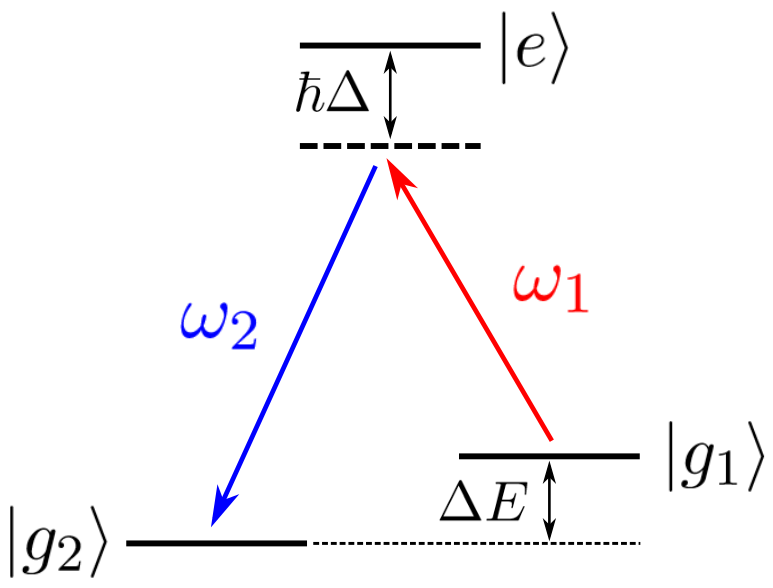
\includegraphics[width=0.5\textwidth]{Fig/Chapter3/raman_level.png}
    \caption{Caption}
    \label{fig:raman_level}
\end{figure}


Importantly, the detuning $\Delta=(\omega_{e}-\omega_{g_1})-\omega_1=(\omega_{e}-\omega_{g_2})-\omega_2$ (see Fig.-\ref{fig:raman_level}) must be large to avoid one photon absorption, {\it i.e.} population of the excited state and spontaneous emission. In these conditions, the excited level can be adiabatically eliminated to describe the two-photon transfer as an effective two-level coupling between $\ket{g_1}$ and $\ket{g_2}$. The system then undergoes well-known Rabi oscillations of frequency:

\begin{equation}
    \Omega_{\rm{eff}}= \sqrt{\frac{\Omega_1^2 \Omega_2^2}{4 \Delta^2} + \delta_{\rm{2p}}^2}
\end{equation}

\noindent where $\Omega_1$ and $\Omega_2$ are the Rabi frequencies associated to laser fields 1 and 2 and $\delta_{\rm{2p}}$ is the detuning to the two-photon resonance condition $\delta_{\rm{2p}}=(\omega_{g_2} - \omega_{g_1}) - (\omega_2-\omega_1)$. The maximum transfer efficiency is the ratio $\eta_{\rm{2p}}=\Omega_{\rm{2p}}^2 /\Omega^2_{\rm{eff}}$ where $\Omega_{\rm{2p}}=\frac{\Omega_1 \Omega_2}{2 \Delta}$ is the effective two-photon Rabi frequency. For $\delta_{\rm{2p}}=0$, we get $\eta_{\rm{2p}}=1$ meaning that it is possible to transfer the entire population of $\ket{g_1}$ to $\ket{g_2}$.

\subsubsection{Experimental implementation}

To implement the two-photon Raman transfer, we use the transition $2 \ ^3 S_1 \rightarrow 2 \ ^3 P_0$ that effectively realize the lambda structure required for Raman transfer (see Fig.-\ref{fig:raman_He}). The pump beam is $\sigma_-$ polarized and the Stokes beam $\pi$ polarized. Importantly, the momentum of the atom is modified because of the absorption of a pump photon and the emission of a Stokes photon. As we do not want to not want to modify the momentum of the atoms during the TOF to properly measure the in-trap momentum, we opt for a configuration with co-propagating beams.

\begin{figure}
    \centering
    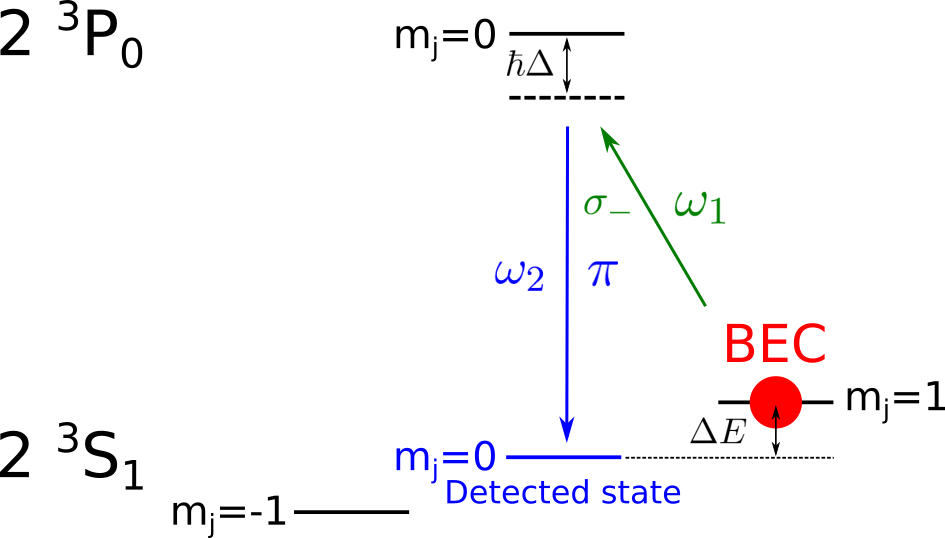
\includegraphics[width=0.7\textwidth]{Fig/Chapter3/raman_exp.png}
    \caption{Implementation of the two-photon Raman transfer with $^4 \rm{He}^*$.}
    \label{fig:raman_He}
\end{figure}

The optical setup is represented in Fig.-\ref{fig:raman_table}. In brief, the two beams are obtained from a single homemade External-Cavity Diode Laser, locked on the $2 \ ^3 S_1 \rightarrow 2 \ ^3 P_0$ of frequency $\nu_0$ via saturated absorption spectroscopy. Actually, in the saturated absorption spectroscopy arm of the setup, the frequency of the laser is shifted by $400 \ \rm{MHz}$ by a double pass Acousto-Optic Modulator (AOM) before locking (see Fig.-\ref{fig:raman_table}), meaning that the frequency of the laser is $\nu = \nu_0 - 400 \ \rm{MHz}$. The main beam is then split in two beams whose respective power are controlled by rotating a half-wave plate in front of a polarizing beam-splitter cube. The frequencies of each beam is set by another double pass AOM. In the end, the frequencies are $\nu_{\rm{Stokes}} = \nu_0 - 800 \ \rm{MHz}$ for the Stokes beam and $\nu_{\rm{Pump}} = \nu_0 - 813 \ \rm{MHz}$ for the pump beam. The small difference of $13 \ \rm{MHz}$ is set to match the energy difference $\Delta E$ between the sub-states $m_J=0$ and $m_J=1$ that we control by applying a magnetic bias field along the $x$ direction. The detuning to the one-photon transition is then $|\Delta|=800 \ \rm{MHz}$ which is large enough to avoid spontaneous emission effects. The polarizations of the two beams are set to be linear and orthogonal. They are finally sent on two faces of a polarizing beam-splitter cube to be overlapped and coupled into a polarization-maintaining fiber bringing them to the science chamber as illustrated on Fig.-\ref{fig:raman_sc}.

\begin{figure}
    \centering
    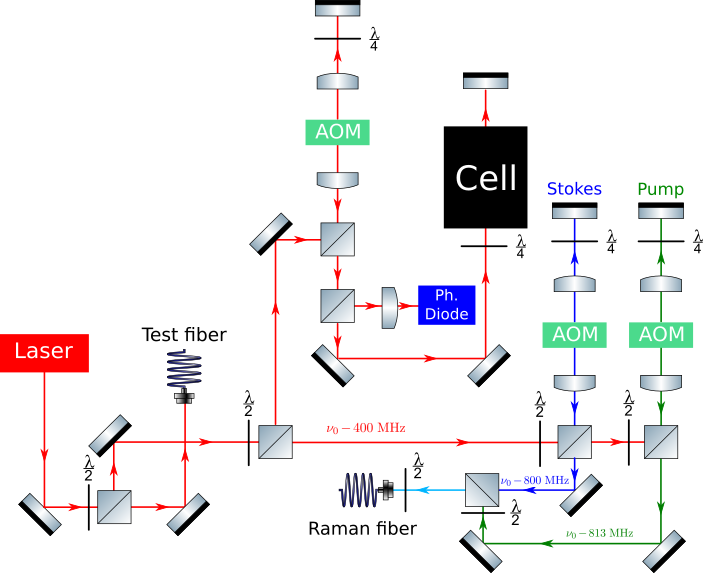
\includegraphics[width=\textwidth]{Fig/Chapter3/table_raman.png}
    \caption{Optical setup for two-photon Raman transfer. After being frequency locked via saturated absorption spectroscopy, the laser beam is split to produce the Stokes and pump beam. The powers are controlled with half-wave plates and polarizing beam splitter, while the frequencies are controlled with Acousto-Optic Modulators.}
    \label{fig:raman_table}
\end{figure}

The polarization at the exit of the fiber is set by a half-wave plate so that the Stokes beam is linearly polarized along the quantification axis $x$ to have the $\pi$ polarisation. The pump beam is linearly polarized as well but orthogonal to the Stokes beam polarisation. This decomposes as the sum of a $\sigma_+$ and $\sigma_-$ polarisation for the atoms. Because of the energy levels structure, the $\sigma_+$ component does not interact with the atom, leaving only the effect of the wanted $\sigma_-$ polarization. This means however than half of the power of the pump beam is useless, requiring to put twice more power for the pump beam than for the Stokes beam for a symmetric configuration.


\begin{figure}
    \centering
    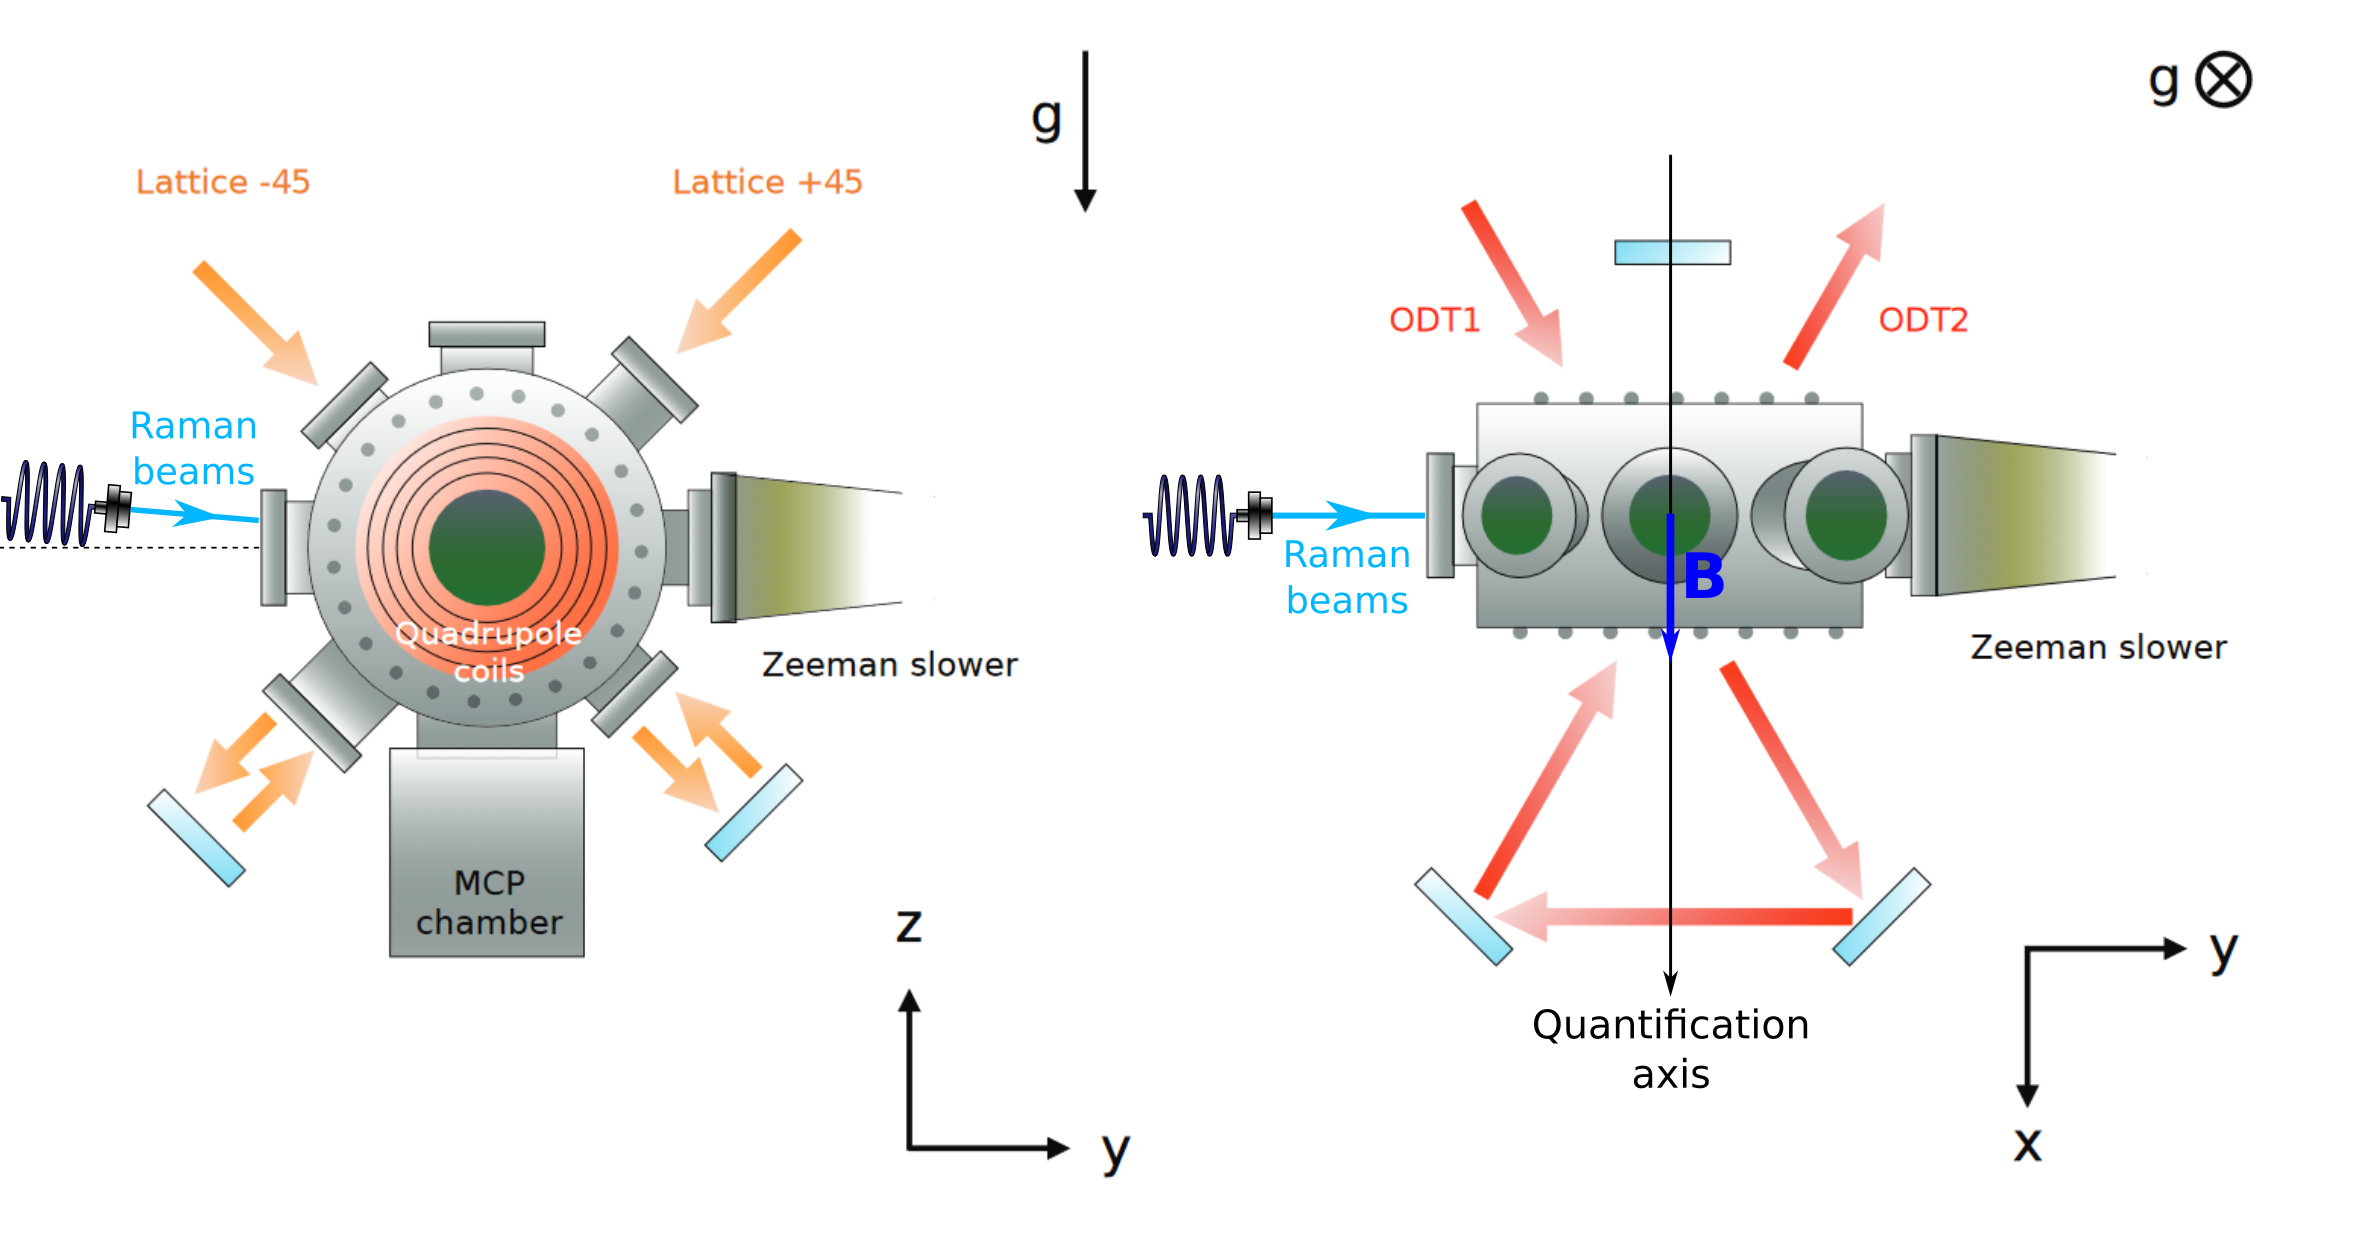
\includegraphics[width=\textwidth]{Fig/Chapter3/raman_sc.png}
    \caption{Orientation of the Raman beams in the experiment. On the right picture, the blue arrow denotes the orientation of the magnetic bias field, setting the quantification axis.}
    \label{fig:raman_sc}
\end{figure}

\subsubsection{Measurement of the two-photon resonance}

As previously discussed, the transfer efficiency is highly dependent from the detuning to the two-photon resonance condition set by the frequency difference $\Delta \nu = \nu_{\rm{Stokes}} - \nu_{\rm{Pump}}$ that we adjust thanks to the pump \NOTE{?} beam AOM. It is therefore important to scan $\Delta \nu$ prior to any use of two-photon Raman transfer to set it perfectly on resonance. The procedure is the following:

\begin{itemize}
    \item We significantly reduce the power of the Raman beams ($30 \ \mu \rm{W}$ and $60 \ \mu \rm{W}$ before the fiber for the Stokes and pump beams respectively) to avoid power broadening of the transition and to have a small Rabi frequency. The period of the Rabi oscillations is then large, we can therefore use a pulse long enough to obtain the necessary frequency resolution, but short enough so that we remain in the first Rabi oscillation when the detuning changes. We chose a pulse duration of $60 \ \mu \rm{s}$ while the Rabi oscillation period is $\sim 200 \ \mu \rm{s}$.
    \item We prepare a Mott insulator whose large momentum distribution prevents saturation effects of the detector from happening.
    \item We perform two-photon Raman transfer for different values of $\Delta \nu$ and plot the number of detected atoms by the MCP as a function of $\Delta \nu$. We finally fit the data to find the position of the resonance as illustrated on Fig.-\ref{fig:raman_resonance}.
\end{itemize}



\begin{figure}
    \centering
    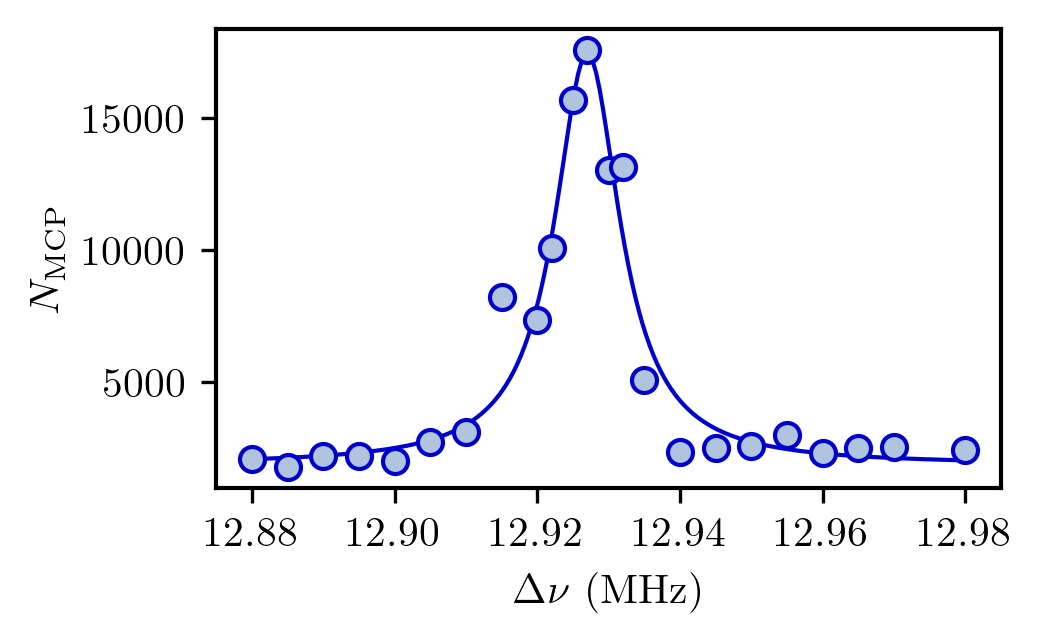
\includegraphics[width=0.7\textwidth]{Fig/Chapter3/raman_res.png}
    \caption{Number of detected atoms $N_{\rm{MCP}}$ (equivalent to the number of transferred atoms) as a function of the frequency difference between the Stokes and pump beams $\Delta \nu$. The maximum of $N_{\rm{MCP}}$ signals the two-photon resonance. The Lorentzian fit gives $\Delta \nu_{\rm{res}} = 12.9270(4) \ \rm{MHz}$.}
    \label{fig:raman_resonance}
\end{figure}

\subsubsection{Rabi oscillations}

In order to check that the two-photon Raman transfer is working as intended, we measure Rabi oscillations for different power values and check that the square Rabi frequency indeed scales linearly with the product of the powers of the Stokes and pump beams. Like when we measure the two-photon resonance, we perform the measurement on a Mott insulator to avoid saturation. The results are shown on Fig.-\ref{fig:rabi_flop} and are consistent with our expectations.

\begin{figure}
    \centering
    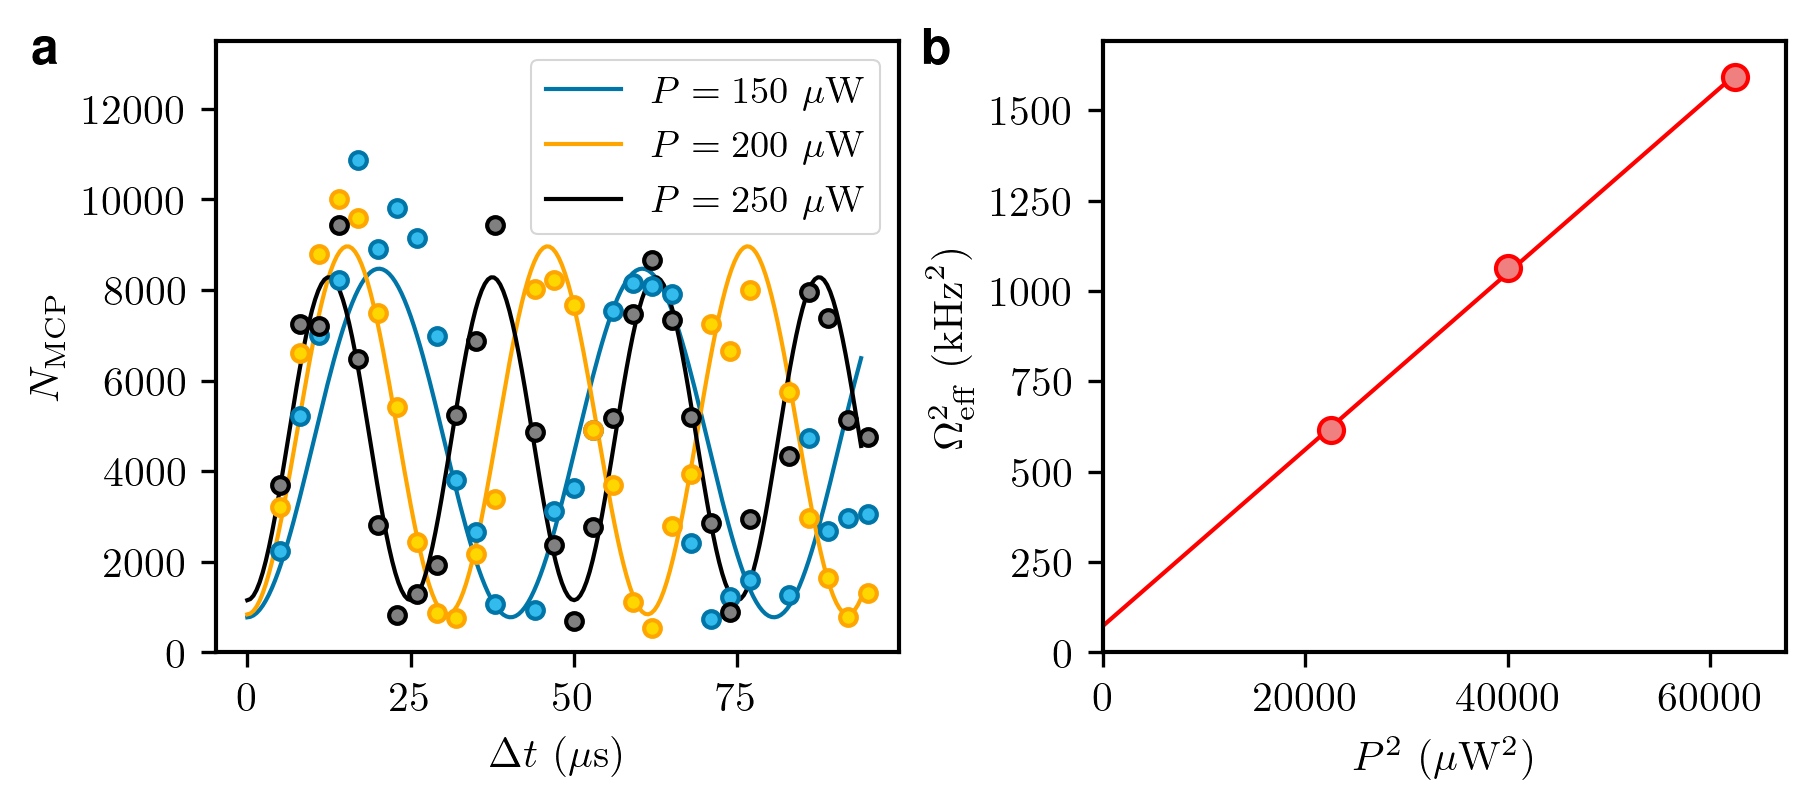
\includegraphics[width=\textwidth]{Fig/Chapter3/rabi_flop.png}
    \caption{Rabi oscillations with two-photon Raman transfer. (a) Rabi oscillations at various beam power. $P$ is the power of the Stokes beam measured before the fiber linking the optical table to the experiment. (b) Square Rabi frequencies $\Omega^2_{\rm{eff}}$ as a function of the square power P (the power of the Stokes and pump beams are set to be the same). We obtain a linear relation with a small offset that might come from a slight miscalibration of the two-photon resonance.}
    \label{fig:rabi_flop}
\end{figure}

Measuring Rabi oscillations is the second part of the procedure to properly set up the two-photon Raman transfer prior to data taking. We set the power of the beams so that the maximum of the first Rabi oscillation corresponds to a pulse duration $t_{\rm{Rabi}} \simeq 10 \ \mu \rm{s}$ and measure a few Rabi oscillations to check it experimentally. This time is chosen to be as short as possible within the resolution of our sequencer so that the transfer efficiency is not sensitive to the fluctuations of the magnetic field as well as its inhomogeneity. Indeed, the bias field that we produce is not perfect, resulting in the presence of a small gradient of $0.17 \ \rm{G/cm}$. If the transfer takes too much time to complete, the atoms have time to travel on a significant distance so that they might see different values of the magnetic field, hence changing the two-photon resonance condition and reducing the overall transfer efficiency.

\subsection{Measurement of the detection efficiency}

\label{sec:detection_efficiency}

We now look to determine the detection efficiency of the $\He$ detector. In a first naive approach, we could simply produce a BEC, measure its number of atoms $\NBEC$ through the well-calibrated absorption imaging, use the two-photon Raman transfer to transfer all the atoms to the $m_J=0$ state, perform the TOF and count the numbers of atoms detected on the MCP $N_{\rm{MCP}}$. The detection efficiency is then simply the ratio $\alpha_{\rm{MCP}}= N_{\rm{MCP}}/\NBEC$. This method would however considerably underestimate the detection efficiency because of the saturation effects occuring with the high densities of the BEC. One could then think of using gases with more dilute distributions to avoid saturation, such as thermal gases or Mott insulators. This method is not so easy as well as it is practically difficult to obtain a momentum distribution wide enough so that the maximum densities values does not saturate the detector, but not too wide to avoid that a significant fraction of the atoms fall beyond the limits of the MCP.

To circumvent these issues, we will then work with a BEC but deliberately use the two-photon Raman transfer with a large detuning to the two-photon Raman transition to transfer only a very small fraction of the atoms and avoid saturation. Using the results of \ref{sec:raman}, the number of detected atoms on the MCP writes:

\begin{equation}
    N_{\rm{MCP}}=\NBEC \left(\frac{\Omega_{2 p}}{\Omega_{\rm{eff}}}\right)^{2} \sin ^{2}\left(\frac{\Omega_{\rm{eff}}  \Delta t}{2}\right) \alpha_{\rm{MCP}}
\end{equation}

\noindent with  $\Omega_{\rm{eff}}= \sqrt{\Omega_{2p}^2 + \delta_{\rm{2p}}^2}$ and $\Delta t$ the duration of the Rabi pulse. If we measure $N_{\rm{MCP}}$, $\NBEC$, $\Omega_{2p}$ and the value of the detuning  $\delta_{2p}$, it is in principle possible to obtain the value $\alpha_{\rm{MCP}}$. We then devise the procedure to measure the detection efficiency to be as follows

\begin{enumerate}
    \item We first need to pinpoint very precisely where the two-photon resonance is. To do so, we measure the frequency of Rabi oscillations $\Omega_{\rm{eff}}$ with a dilute gas for different values of the frequency difference $\Delta \nu$ between the Stokes and the pump beam close to the two-photon resonance condition. At this point, we do not care about the amplitude of the Rabi oscillations but only their frequency. Using $\Omega_{\rm{eff}}= \sqrt{\Omega_{2p}^2 + \delta_{\rm{2p}}^2}$, we fit the experimental data to find the value of $\Delta \nu$ where $\Omega_{\eff}$ is minimum which corresponds to the two-photon resonance as illustrated on Fig.-XX.
    \item We prepare a BEC of $\NBEC = 2 \times 10^5$ atoms that we calibrate with absorption imaging.
    \item We set the power of the Raman beams to have $\Omega_{\rm{2p}}=20 \ \rm{kHz}$.
    \item We measure Rabi oscillations for various values of $\delta_{\rm{2p}} \in [300,1000] \ \rm{kHz}$ and extract the amplitude of the square sine function $N^{\rm{max}}_{\rm{MCP}}$.
    \item We plot $N^{\rm{max}}_{\rm{MCP}}$ versus $\NBEC \left(\frac{\Omega_{2 p}}{\Omega_{\rm{eff}}}\right)^{2} \alpha_{\rm{MCP}}$. We fit the data with a linear function and deduce the value of $\alpha_{\rm{MCP}}$ from the slope of the fit as illustrated on Fig.-XX \NOTE{to do}.
\end{enumerate}

\noindent The final measured value is \fcolorbox{red}{white}{$\alpha_{\rm{MCP}}=0.53(2)$}. As mentioned earlier, the open-to-air ratio of the MCPs is around $\simeq 90 \%$, meaning that almost all atoms fall in a channel, thus not limiting the detection efficiency. However, the first extracted electron has roughly a 1/2 probability to be ejected upwards outside of the channel, rendering the amplification process impossible, explaining why we observe a detection efficiency of the order of $50 \%$.



\section{Characterisation of two-body collisions in the time-of-flight dynamics}

Before using our experimental setup to look for the \kmk correlations of the quantum depletion, it is crucial to benchmark it and test whether the measured distribution $\rho_{\rm{TOF}} (\bm{r},t_{\rm{TOF}})$ indeed maps the in-trap momentum distribution $\rho(\bm{k})$ or is perturbed by interactions effects occuring during the TOF. In Chapter $\ref{sec:chapter_2}$, we have seen that the interactions can be conveniently treated thanks to the mean-field approximation. Under this approximation, the effects of interactions is expected to be negligible. This hypothesis was verified by comparing the experimental data to Quantum Monte Carlo calculations of the in-trap momentum distribution, obtaining a very good agreement \cite{cayla2018single}. For more details on this measurement, we refer the reader to the previous manuscripts \cite{carcy_these,cayla_these}.

In this section, we will focus on interaction effects that cannot be described by the mean-field approximation, namely \textbf{two-body collisions}, to characterize them and determine whether they perturb the measured distribution or not.

\subsection{Presentation of the problem}

As we have seen in Chapter \ref{sec:chapter_2}, the momentum distribution of the lattice gas in the superfluid region of the phase diagram is made of copies of the BEC of momentum $j k_d \bm{e}_i$ with $j \in \Z$ and $i=x,y,z$. During the TOF, it is possible to observe s-wave collisions between the atoms of these different BEC copies. Let us then for instance consider the case of a collision between an atom in the copy $j=0$ with initial momentum $\bm{k}_{i1}=\bm{0}$ and one in the $x$ copy $j=1$ with initial momentum $\bm{k}_{i2}=k_d \ \bm{e}_x$. If we write these momenta in the center-of-mass reference frame, we rather get $\bm{k}_{i1}=-k_d/2 \ \bm{e}_x$ and $ \bm{k}_{i2}=k_d/2 \ \bm{e}_x$. As the collision is elastic, the momentum and kinetic energy are conserved:

\begin{equation}
    \bm{k}_{i1}+\bm{k}_{i2}=\bm{k}_{f1}+\bm{k}_{f2}=\bm{0}
\end{equation}

\begin{equation}
    \frac{\hbar^2 k^2_{1f}}{2m} + \frac{\hbar^2 k^2_{2f}}{2m} =  \frac{\hbar^2 k_d^2}{2m}
\end{equation}

\noindent This means that $\bm{k}_{1f}$ and $\bm{k}_{2f}$ must have equal norms $k_d/2$ and be antiparallel. Their direction is a priori random. After the collision, the atoms then end up on a sphere of diameter $k_d$ in momentum space as illustrated on Fig.-\ref{fig:schema_collisions}. For a large number of collisions, all the atoms that underwent a collision form a spherical halo that we can observe experimentally.

\begin{figure}[ht!]
    \centering
    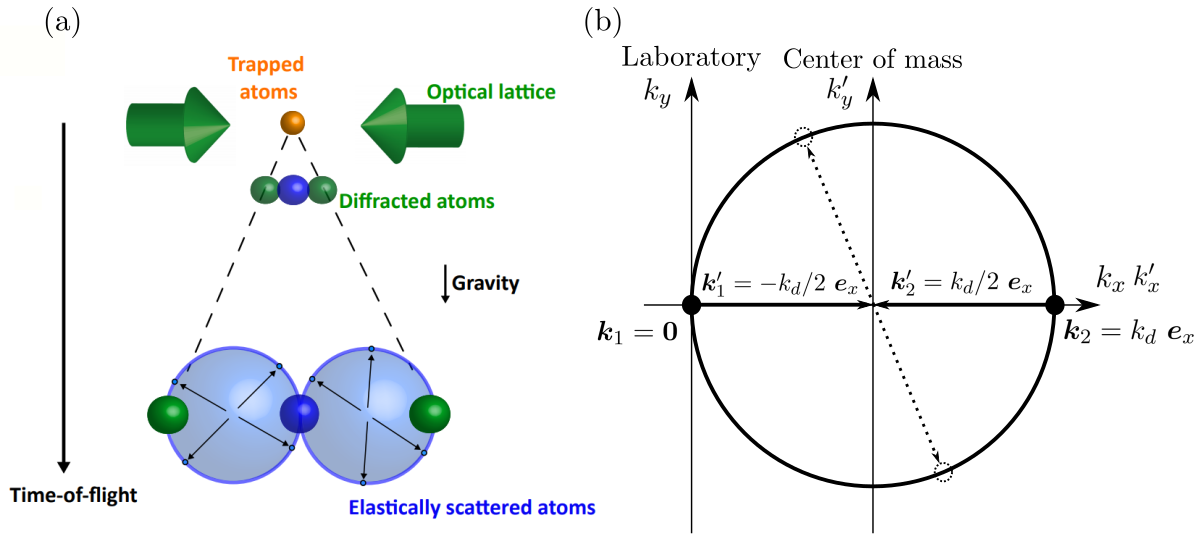
\includegraphics[width=\textwidth]{Fig/Chapter3/schema_collisions.png}
    \caption{Elastic collision between copies of the condensate. (a) Sketch of the experiment in one axis. During the TOF, diffracted copies of the BEC form as a result of the lattice trapping potential. Two-body collisions can occur between these different diffracted copies and manifest themselves as spherical halos. (b) Illustration of the momentum conservation rule explaining the spherical shape of the collision halos.}
    \label{fig:schema_collisions}
\end{figure}

We understand that this effect is detrimental to our measurement, as the collision process changes the momentum distribution of the gas during the TOF, meaning that we do not measure the true in-trap momentum distribution. However, the collision halos are not visible for the low atom numbers we wish to work with for the observation of the \kmk pairs of the quantum depletion. While this is a good sign, we would like to know precisely how likely it is for a two-body collision to happen in these conditions so that we can safely apply the ballistic relation. We will then deliberately load a large number of atoms in the optical lattice to observe clear collision halos and count the number of atoms inside of them in order to validate a simple classical model that we will use to predict the number of collisions at the low atom numbers we wish to use.

\subsection{Classical model}

We will start our study by devising a simple classical model to evaluate the number of collisions before checking its validity experimentally. To illustrate the idea behind it, we compute the number of collisions between the condensate copies $j=0$ and $j=1$. The first step is to evaluate the collision rate of one atom a position $\bm{r}$ at time $t$ belonging to the BEC copy with all the atoms in the copy $j=1$. This rate writes \cite{chikkatur2000suppression,perrin:tel-00244641}:

\begin{equation}
    \Gamma_{\text {coll }}=n_{1}(\bm{r}, t) \times \sigma \times v_{0,1}
\end{equation}

\noindent where $n_1$ is density of the copy $j=0$, $v_{0,1}=v_d=\hbar k_d/m$ the relative velocity of the two copies and $\sigma= 8 \pi a_s^2$ the scattering cross-section, with $a_s$ the s-wave scattering length ($a_s = 142 a_0$ for $^4\He$ with $a_0$ the Bohr radius). To obtain the total number of collisions, we integrate over all particles of the copy $j=0$ and over the time interval during which the copies spatially overlap. If we wish to obtain the number of collisions for all first order copies, we can simply multiply this number by $6$ to finally obtain:

\begin{equation}
    N_{\text {coll }}=6 \int d t \int d \bm{r} \ \sigma v_{d} n_{0}(\bm{r}, t) n_{1}(\bm{r}, t)
    \label{eq:coll_model_general}
\end{equation}

To evaluate this quantity, we need to determine the density profiles $n_{j}(\bm{r}, t)$. While a full description of the TOF dynamics would be way to complicated in the frame set by this simple model, the densities can be evaluated by considering the different energies and time scales of the problem. The shortest time scale is set by the frequency of a lattice site $\omega_{\rm{site}}$ to which we associate the corresponding harmonic oscillator length $a_{\text {h.o. }}=\sqrt{\hbar / m \omega_{\text {site }}}$. From this, we compute the time scale $t_0 \simeq m d a_{\text {h.o. }} /h \simeq 1 \ \mu \rm{s}$ on which the wave-functions of the different sites overlap. After a few $t_0$, the overall density profile is smoothed with a total size hardly larger than the in-trap size $L$ and a lower density than that in the trap. In turn, the densities profile are then well described by the Thomas-Fermi parabolic profile of the BEC $n_{\rm{BEC}}(\bm{r})$.

We now need to consider the other timescales, much larger than $t_0$ and associated with:

\begin{itemize}
    \item The spatial separation of two copies $t_{\rm{sep}} \sim 2L/v_d \sim 0.1 \ \rm{ms}$.
    \item The expansion of the BEC driven by its kinetic energy $t_{\mathrm{kin}} \sim m L / \hbar \Delta k \sim 10 \mathrm{~ms}$ where $\Delta k$ is the momentum width of the BEC.
    \item The expansion of the BEC under the effect of the mean-field potential $t_{\rm{MF}}$.
\end{itemize}

\noindent We notice that when the size of the trapped gas is much larger than the lattice spacing $L \gg d$ which is typically the case in our experiment, we get $\Delta k \ll k_d$ explaining why we obtain $t_{\rm{sep}} \ll t_{\rm{kin}}$. Things are more complicated for $t_{\rm{MF}}$ as it depends on the number of atoms and can be of the order of $t_{\rm{sep}}$. From this, we consider two scenarios: one where the number of atoms is small enough so that mean-field effects can safely be neglected, and one where they must be accounted for.

\subsubsection{Scenario 1: mean-field effects are negligible}

In this scenario, the size of the BEC copies increases in time only through the effect of kinetic energy. As we have seen that $t_{\rm{sep}} \ll t_{\rm{kin}}$, we understand that the size of the density profiles hardly changes during the interaction time, \ie before separation of the different BEC copies. We can therefore safely assume that the shape of the densities profile does not change during the interaction time, allowing us to evaluate analytically equation \ref{eq:coll_model_general} to obtain:

\begin{equation}
    N_{\text {coll }}=\frac{48 \alpha_{0} \alpha_{1}}{315}\left(\frac{15 N_{\text {bec }} a_{s}}{L}\right)^{2}
    \label{eq:analytical_model}
\end{equation}

\noindent where we have introduced the coefficients $\alpha_j$ denoting the fraction of the total atom number in one of the copies $j$. The scaling $N_{\text {coll }} \propto a_{s}^{2} N_{\text {bec }}^{2} / L^{2}$ is identical to what was found in previous works describing the collisions between two BECs \cite{zin2005quantum,zin2006elastic}. 

\subsubsection{Scenario 2: mean-fields effects are not negligible}

In this scenario, it is not possible anymore to assume that the shape of the density profiles does not change during the interaction time, making the calculation of equation \ref{eq:coll_model_general} much more complicated and beyond the scope of this thesis. This is however not really important as the goal of this experiment is to determine the number of collisions at low atom number. If we are able to find atom numbers for which the collisions spheres are visible while the mean-field effects are negligible, we will be able to validate our simple model and use it to predict the number of collisions at low atom numbers. We must however keep in mind that the analytical model of equation \ref{eq:analytical_model} should fail at high atom numbers. The expansion of the BEC copies induced by the mean-field effects implies a decrease of the density compared to Scenario 1, meaning that we should observe less collisions that what is predicted from equation \ref{eq:analytical_model}.

Actually, it is possible to discriminate between the two scenarios rather easily by looking at the width of the collision spheres. When the expansion is ballistic, \ie in Scenario 1, the width of the collision sphere that we will note $\delta k_s$ is equal to the in-trap momentum width $\Delta k \propto 1/L$ and should therefore decrease when the total number of atoms increases. On the contrary, $\delta k_s$ is increased in Scenario 2 because of the additional kinetic energy resulting from the mean-field interaction potential, meaning that $\delta k_s$ increases when the strength of mean-field effects increases, \ie when the atom number increases. We therefore expect the variations of $\delta k_s$ with the total atom number $N_{\rm{BEC}}$ to show a minimum that signals the crossover between Scenarios 1 and 2.

\subsection{Data analysis}

We show on Fig.-\ref{fig:spheres} the typical detected momentum distribution on which we can see clear collision halos. We produce a variety of data sets to test the effect of the atom number and of the lattice amplitude. The procedure to count the number of collisions is as follows:

\begin{enumerate}
    \item For each collision halo, we restrict the analysis to a small slice so that we exclude the region where the halo intersects with the condensate peaks or other collision halos as illustrated on the inset of the Fig.-\ref{fig:sphere_profiles}. 
    \item We calculate for each atom in the slice the momentum distance to the center of the sphere $k_r$ and compute the histogram $\mathcal{N}(k_r)$ of the number of atoms located at a distance $k_r$. The size of the bins is $0.01 \ k_d$.
    \item We account for the efficiency of our detection process $\alpha_D$ by multiplying the value of each bin of the histogram by $1/\alpha_D$. Careful, as this experiment was done before the implementation of the Raman transfer, the efficiency was lower than measured in \ref{sec:detection_efficiency}. A full calibration as the one previously described was not possible as we could not observe clean Rabi oscillations because of the much smaller Rabi frequencies. We therefore measured $\alpha_D$ by recording diluted distributions of Mott insulators to avoid saturation effects and comparing them to absorption images for which we can precisely know the number of atoms. We obtained $1/\alpha_D=15.5(1.0)$.
    \item We obtain histograms such as represented on Fig.-\ref{fig:sphere_profiles} in which we observe a peak at $k_r=0.5 \ k_d$ signalling the presence of the collision halo. We remove the contribution of the background that corresponds to the quantum and thermal depletion and fit the peak with a Gaussian function to obtain the width of the halo $\delta k_s$ and the number of atoms in the slice of collision halo.
    \item Assuming spherical symmetry, the total number of scattered atoms is obtained by integrated the value measured in the slice over the entire sphere. 
    \item We finally obtain the number of detected collisions $N_{\rm{coll}}^{\rm{exp}}$ by summing the number of scattered atoms measured in the different halos. Note that we use only 5 of the 6 first order halos as one of them is partially falling out of the MCP. 
\end{enumerate}

\begin{figure}
    \centering
    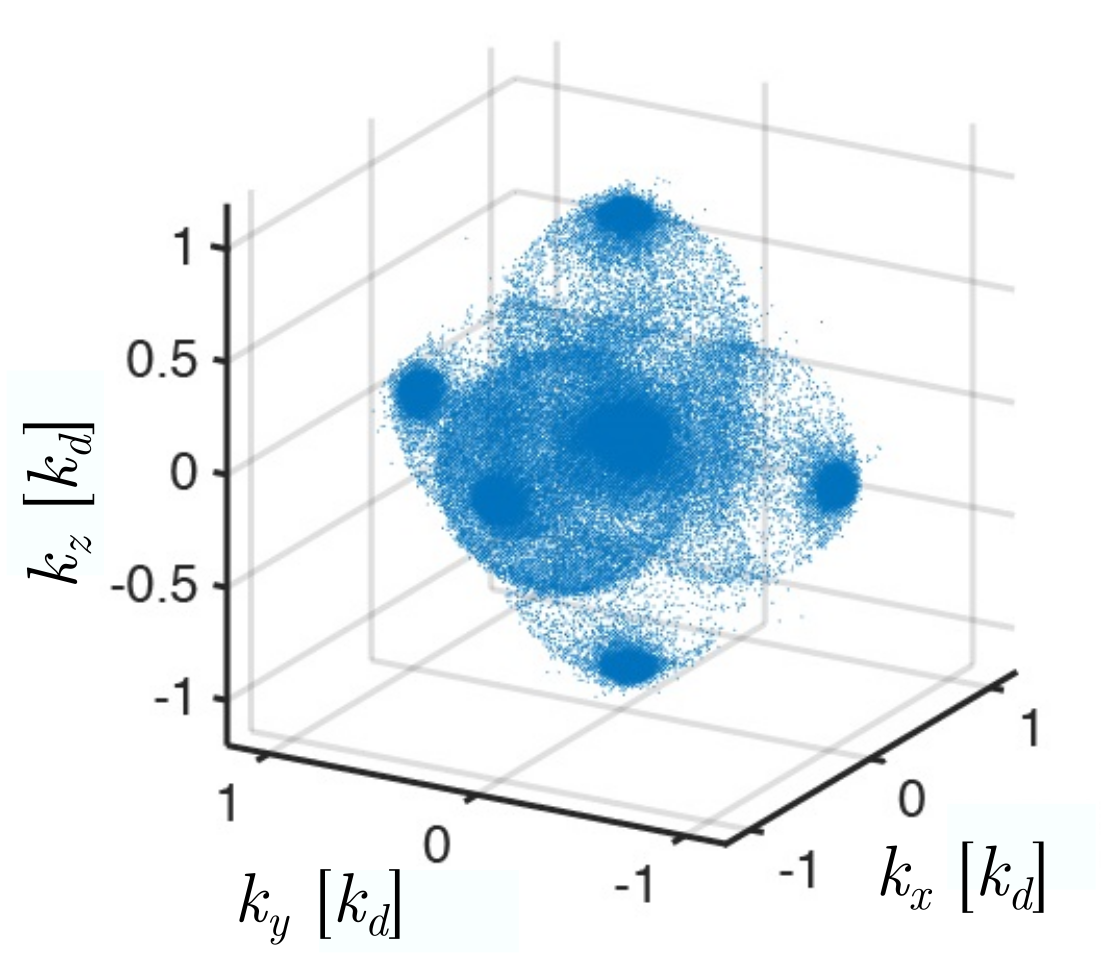
\includegraphics[width=0.6\textwidth]{Fig/Chapter3/spheres.png}
    \caption{3D momentum distribution of a superfluid lattice gas. The $s$-wave scattering halos are clearly visible.}
    \label{fig:spheres}
\end{figure}

\begin{figure}
    \centering
    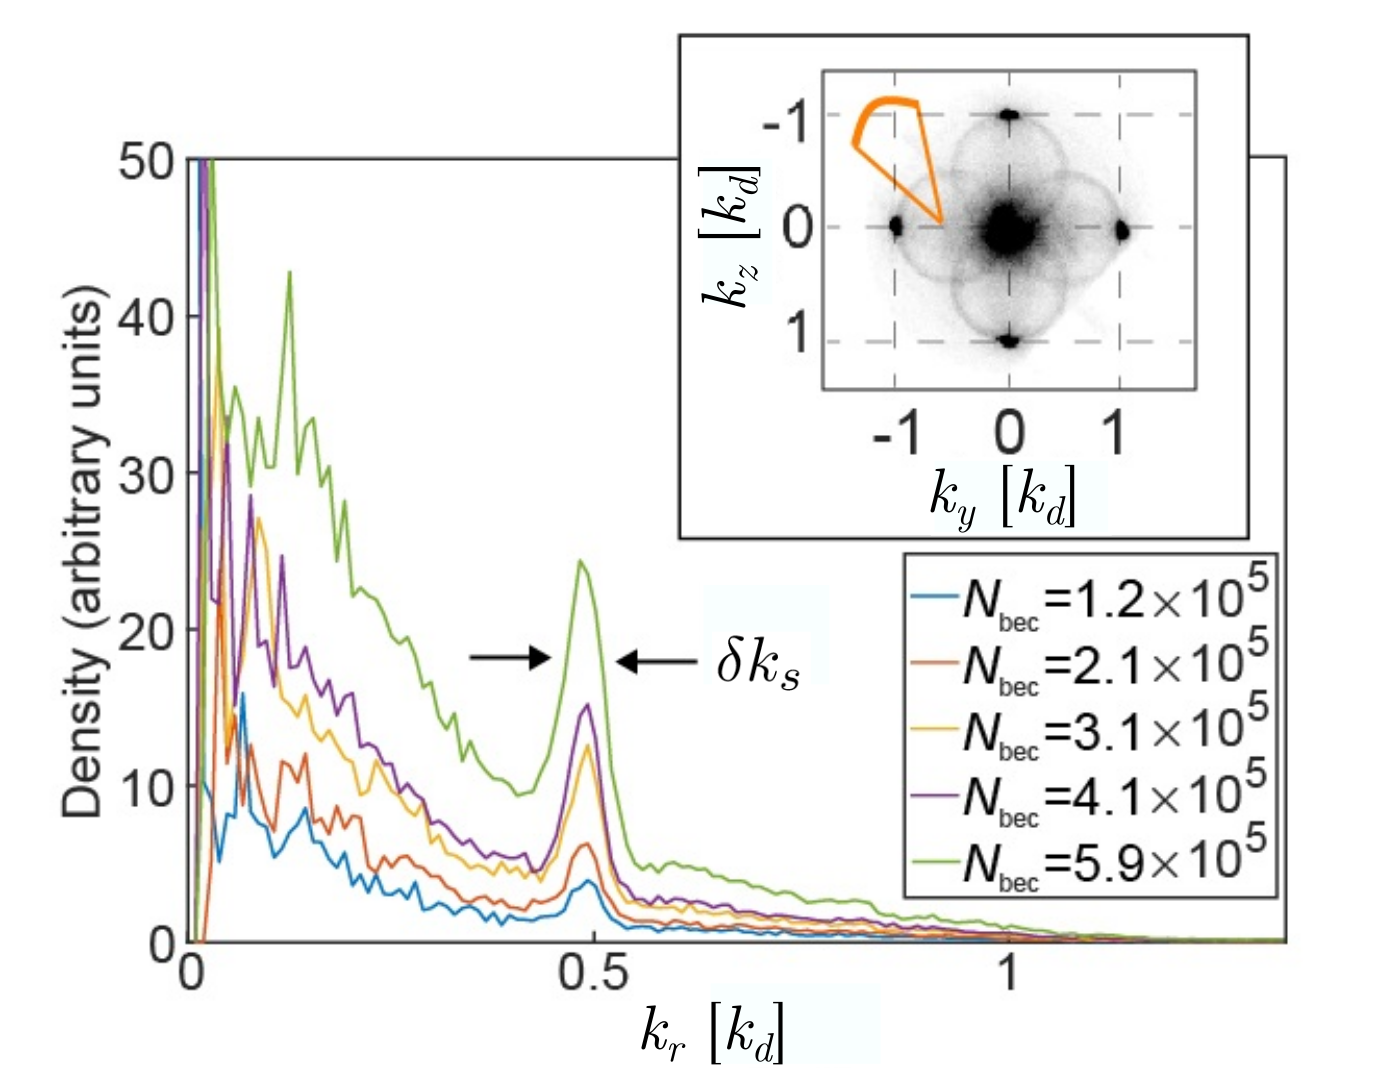
\includegraphics[width=0.7\textwidth]{Fig/Chapter3/sphere_profiles.png}
    \caption{Atom numbers histograms as a function of the momentum distance $k_r$ to the center of the collision halo. We show histograms for different total atom numbers $\NBEC$ for a fixed lattice amplitude $s=5$. Inset: two-dimensional cut at $k_x=0$ through the 3D distribution. The orange region indicates where the number of scattered atoms is calculated.}
    \label{fig:sphere_profiles}
\end{figure}

\subsubsection{Width of the collision halos}

We show on Fig.-\ref{fig:largeur_spheres} the measured RMS widths of the collision halos $\delta_s$ as a function of the atom number. The error bars are obtained from the error on the Gaussian fit. As expected, we observe a minimum around $N_0 \simeq 1.7 \times 10^5$ at which the mean-field effects start playing a role. 

\begin{figure}
    \centering
    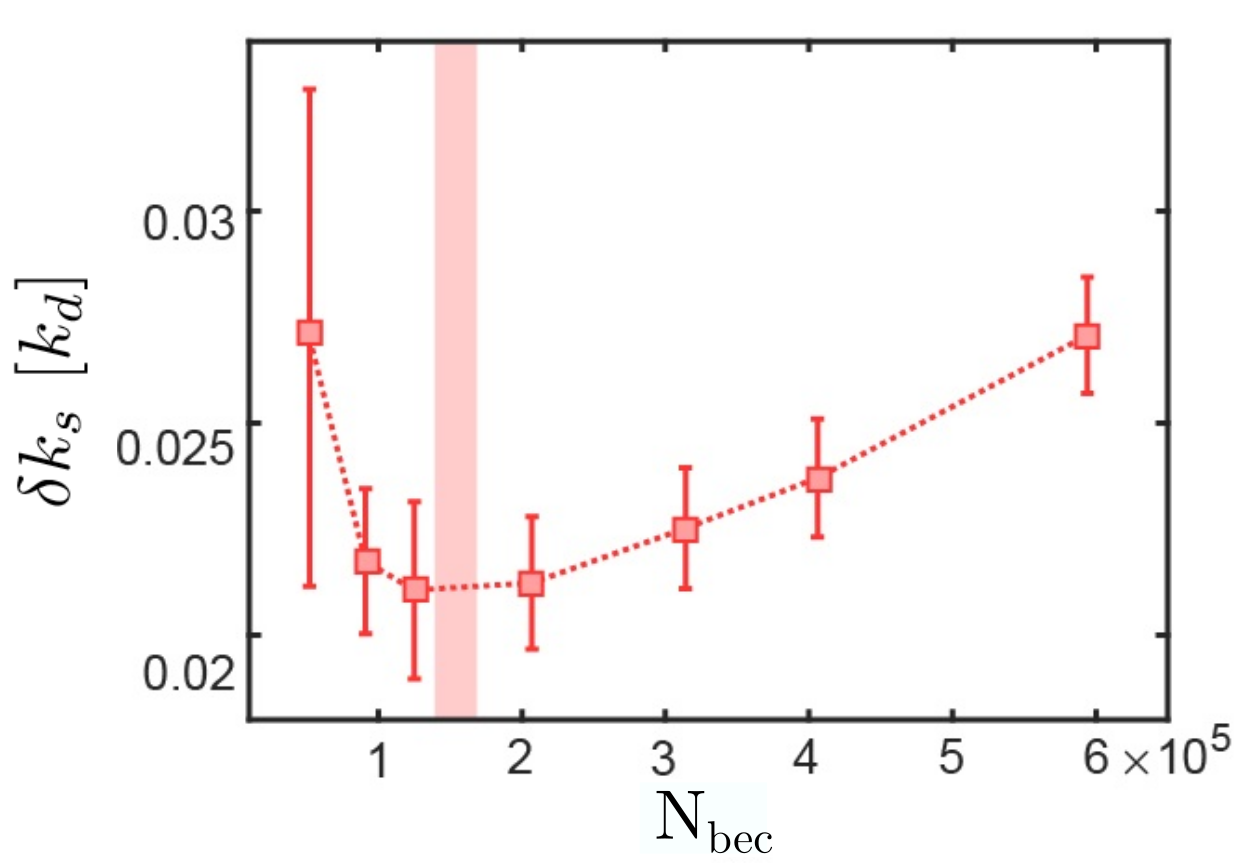
\includegraphics[width=0.6\textwidth]{Fig/Chapter3/largeur_spheres.png}
    \caption{RMS width $\delta k_s$ of the scattering halos as a function of $N_{\rm{bec}}$. The red dashed line is a guide-to-the-eye. The red shaded area signals the crossover between the two scenarios described in the main text.}
    \label{fig:largeur_spheres}
\end{figure}

\subsubsection{Evolution with total atom number}

We plot on Fig.-\ref{fig:ncoll_vs_atom_number} the evolution of the number of collisions with the total atom number at a fixed lattice amplitude $s=5$. The vertical error bars account for the standard error of the mean on $N_{\rm{coll}}^{\rm{exp}}$ and the uncertainty on the detection  efficiency. The horizontal error  bars depict the standard deviation on $N_{\rm{bec}}$. The dashed line represents the analytical model of equation \ref{eq:analytical_model} where the effect of the atom number is contained in the term $(\NBEC/L)^2$ giving in the Thomas-Fermi approximation $N_{\rm{coll}} \propto \NBEC^{8/5}$. While we find a good agreement with the experimental data at low atom number and without any adjustable parameters, we find that the analytical model overestimates the number of collisions for $\NBEC > N_0$ as expected. In addition, we plot the probability of collision per atom $\eta_1=N_{\rm{coll}}^{\rm{exp}}/N_{\rm{bec}}$.

\begin{figure}
    \centering
    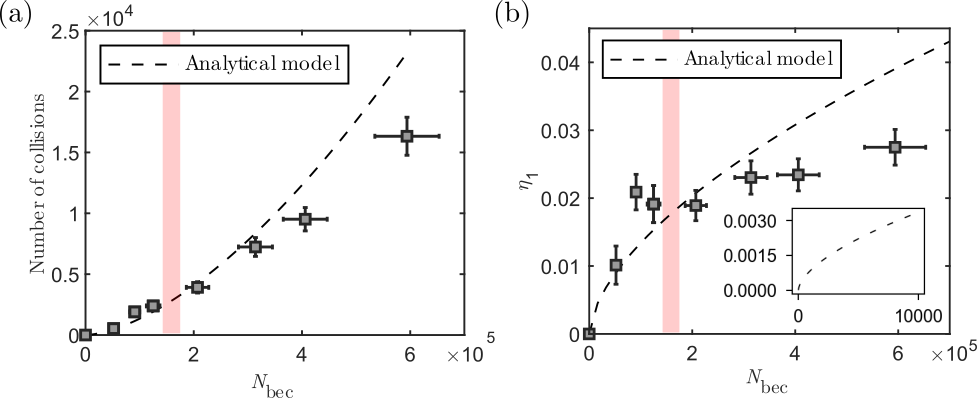
\includegraphics[width=\textwidth]{Fig/Chapter3/ncoll_vs_atom_number.png}
    \caption{(a) Experimental number of collisions $N_{\rm{coll}}^{\rm{exp}}$ between the copies $j=0$ and $j=1$ as a function of the atom number $\NBEC$ at a fixed lattice amplitude $s=5$. The dashed line is the analytical model of equation \ref{eq:analytical_model}. (b) Probability of collision per atom $\eta_1=N_{\rm{coll}}^{\rm{exp}}/N_{\rm{bec}}$.}
    \label{fig:ncoll_vs_atom_number}
\end{figure}

\subsubsection{Evolution with lattice depth}

 We plot on Fig.-\ref{fig:ncoll_vs_s} the evolution of the number of collisions with the lattice amplitude $s$ at a fixed total number of atoms $\NBEC = 3.9(4) \times 10^5$. As we have seen in Chapter \ref{sec:chapter_2}, the lattice amplitude changes the population of the BEC copies and therefore the coefficients $\alpha_0$ and $\alpha_1$ appearing in \ref{eq:analytical_model}. At very low lattice amplitudes, the population in the diffracted peaks is very small, $\alpha_0 \simeq 1$, $\alpha_1 \simeq 0$, meaning that the number of collisions is very low. As $s$ increases, the number of collisions increases as $\alpha_1$ increases. With $s > 5$, we start populating higher orders of diffraction, thus reducing the number of collisions between the copies $j=0$ and $j=1$. This explains the non-monotonic behavior of the analytical model that is well reproduced by the experimental data. Once again, the model overestimates the number of collisions as $\NBEC > N_0$.
 
 \begin{figure}
     \centering
     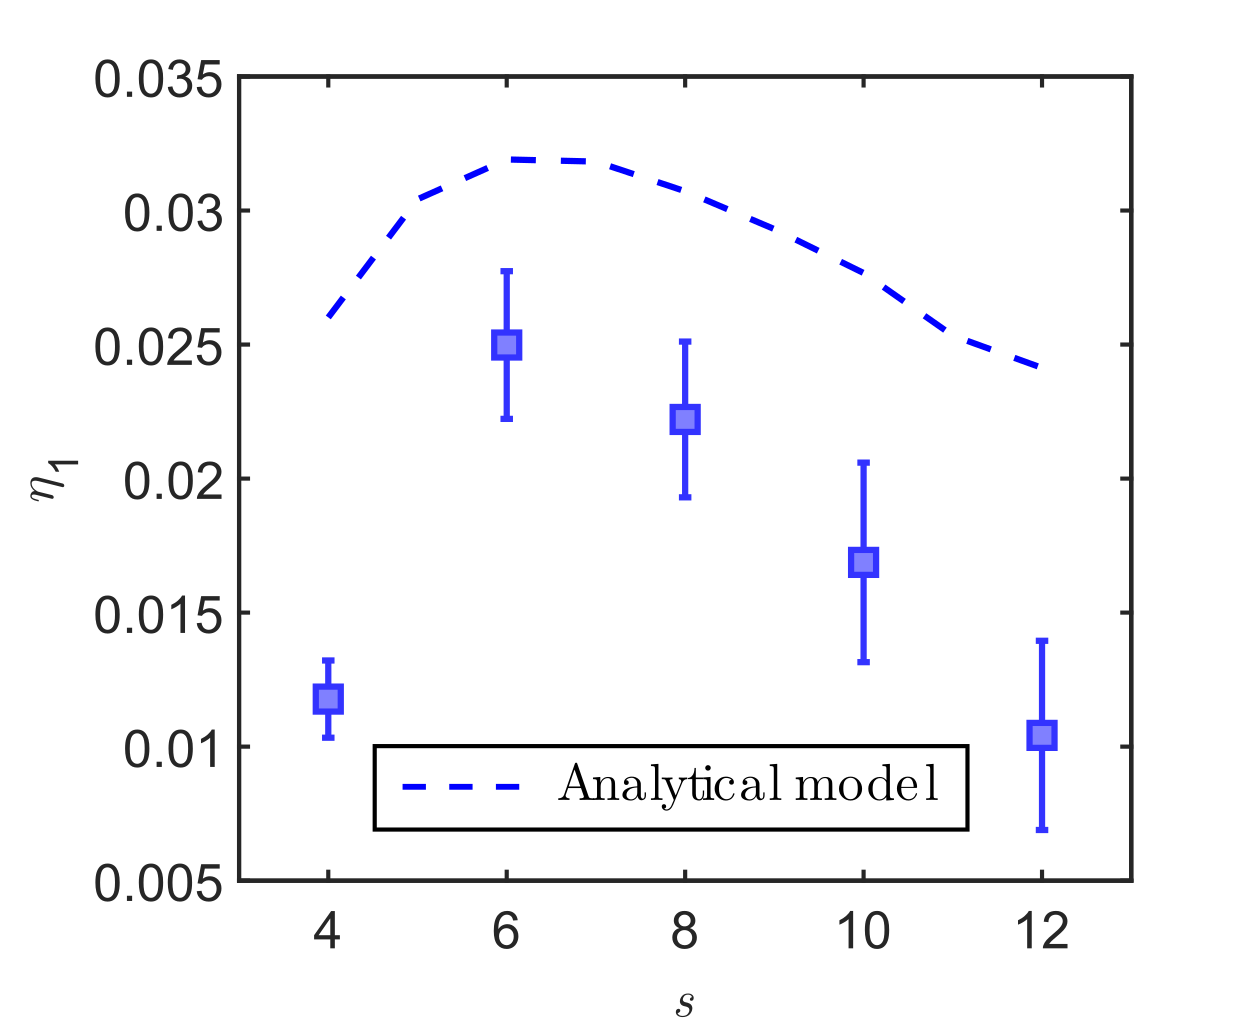
\includegraphics[width=0.6\textwidth]{Fig/Chapter3/ncoll_vs_s.png}
     \caption{Probability of collision per atom $\eta_1$ as a function of $s$ at a fixed atom number $\NBEC=3.9(4) \times 10^5$. The blue dashed line is the analytical model of equation \ref{eq:analytical_model}.}
     \label{fig:ncoll_vs_s}
 \end{figure}

\subsection{Conclusion}

Now that we have validated that our analytical model properly works for low atom number, we can determine the probability of collision per atom for the typical atom numbers that we wish to use for the \kmk correlation experiment. For $\NBEC \sim 5 \times 10^3$, we find as shown on panel b of Fig-\ref{fig:ncoll_vs_atom_number} that the probability for an atom to collide during the TOF is $\eta_1 \sim 10^{-4}$ which is extremely low. Before reaching our final conclusion, we need to discuss the contribution of other possible scattering halos, such as the one involving higher order copies $j \geq 2$ or between two first order copies. These halos are more diluted because of a lower number of collisions and larger volume and are in turn not visible in the experiment, but might contribute significantly at high values of $s$. We can evaluate their contribution by setting the appropriate values of $\alpha_j$ in equation $\ref{eq:analytical_model}$. We obtain an upper bound by considering the extreme situation where the number of copies would be as large as the number of atoms and find that this increases $\eta_1$ by only a factor 3, meaning that the measured probability $\eta_1$ gives a good estimate of the total probability of collisions. We can therefore safely conclude that two-body collisions will be negligible in our \kmk pair experiment. This results completes the previous benchmarking experiments \cite{cayla2018single}, proving that the ballistic relation applies in our experiment.

\section{Adiabatic preparation in the vicinity of the Mott transition}

As developed in the first pages of this thesis, the general objective of our experiment is to simulate quantum interacting systems too complex to treat theoretically. More specifically, our experimental apparatus aims to simulate the equilibrium properties of the Bose-Hubbard many-body ground-state. The standard procedure is to create a non-zero entropy state, the BEC, and progressively transform the Hamiltonian of the system by loading the atoms in the optical lattice to reach the desired Bose-Hubbard state. It is crucial that this transformation does not create excitations populating higher bands: in other terms, we want to keep the entropy of the system constant as we load the atoms in the optical lattice, \ie ensure that the preparation of the target Hamiltonian is \textbf{adiabatic}. 


\subsection{Loading of the optical lattice}

The optical lattice is loaded by ramping down the power of the ODT beams while ramping up the power of the lattice beams. We use several parameters to fine tune the loading sequence as represented on Fig.-\ref{fig:loading}:

\begin{itemize}
    \item The slope of the lattice ramp.
    \item $t_{\rm{down}}$ the time on which we ramp down the ODT power.
    \item $t_{\rm{delay}}$ the time delay between the beginning of the ramp of the optical lattice and the ramp of the ODT.
\end{itemize}

\begin{figure}
    \centering
    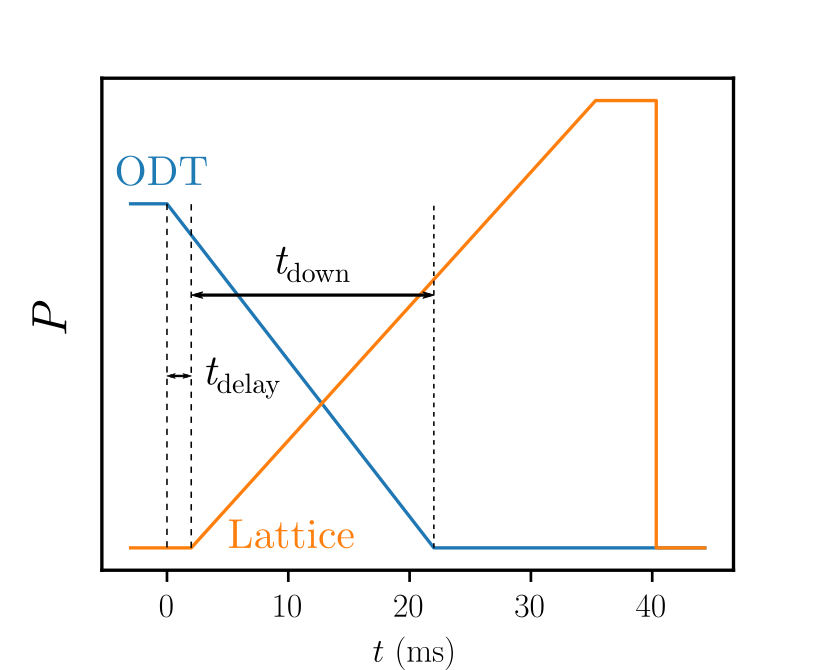
\includegraphics[width=0.7\textwidth]{Fig/Chapter3/loading.png}
    \caption{Loading sequence of the lattice.}
    \label{fig:loading}
\end{figure}

In order to optimize these parameters, the atoms are loaded back in the ODT with a symmetrical sequence to look for atom losses and heating effects to be minimized as illustrated on Fig-\NOTE{to do}. We found that the shape of the ramp were not important and settled for simple linear ramps, corresponding to an almost exponential increase of $s$ (see Fig-\ref{fig:U_J_vs_s}). Their slope was set to $0.3 \ E_{\rm{r}}/\rm{ms}$ and remains constant no matter the final target value of $s$, only the ramp time changes. The optimal values of the other ramp parameters were found to be \fcolorbox{red}{white}{$t_{\rm{down}}=22 \ \rm{ms}$} and \fcolorbox{red}{white}{$t_{\rm{delay}}= 0 \ \rm{ms}$}. With these parameters, we observe a typical $20 \%$ losses that we attribute to the not perfect overlap between the ODT and the lattice, but no heating.

\subsection{Thermometry and entropy across the Mott transition}

Now that we have experimentally optimized the parameters of the loading sequence, we verify the adiabaticity of the loading sequence by extracting the temperature and the entropy from the momentum distribution.

\subsubsection{Thermometry method}

The temperature of the gas cannot be extracted directly from the density $\rho(\bm{k})$ as we do not have an analytical prediction for the trapped Bose-Hubbard model. The idea is then to use ab-initio Quantum Monte Carlo (QMC) calculations simulating the momentum distribution with the only adjustable parameter being the temperature. The QMC calculations were provided by Tommaso Roscilde from the Ecole Normale Supérieure de Lyon and were run for different temperature values. To get the temperature in the experiment, we select the QMC momentum distribution that best reproduces the experimental data  as illustrated in Fig.-\ref{fig:comp_qmc}. Formally speaking, we compare a cut of the normalized experimental density $\tilde{\rho}_{\rm{exp}}(k)=\rho(k,0,0)/\rho(0)$ to the QMC ones $\tilde{\rho}_{\rm{exp}}(k,T)=\rho_{\rm{QMC}}(k,0,0,T)/\rho_{\rm{QMC}}(0)$. We look to find the temperature value that minimizes the reduced chi-square quantity that we define as:

\begin{equation}
    \chi_{\mathrm{r}}^{2}(T)=\frac{1}{N_{p}} \sum_{j=1}^{N_{p}} \frac{\left[\bar{\rho}_{\mathrm{exp}}\left(k_{j}\right)-\bar{\rho}_{\mathrm{QMC}}\left(k_{j}, T\right)\right]^{2}}{\sigma_{\exp }\left(k_{j}\right)^{2}}
\end{equation}

\noindent We have discretized the first Brillouin zones with a uniform mesh of $N_p=120$ points. The quantity $\sigma_{\exp }\left(k_{j}\right)$ is the error estimate on the experimental momentum density that is assumed to have Poissonian statistics, giving us $\sigma_{\exp }\left(k_{j}\right)=\sqrt{\tilde{\rho}_{\exp }\left(k_{j}\right) / N_{\rm{runs}}}$ with $N_{\rm{runs}}$ the number of experimental runs used to evaluate $\tilde{\rho}_{\rm{exp}}(k)$.


\begin{figure}
    \centering
    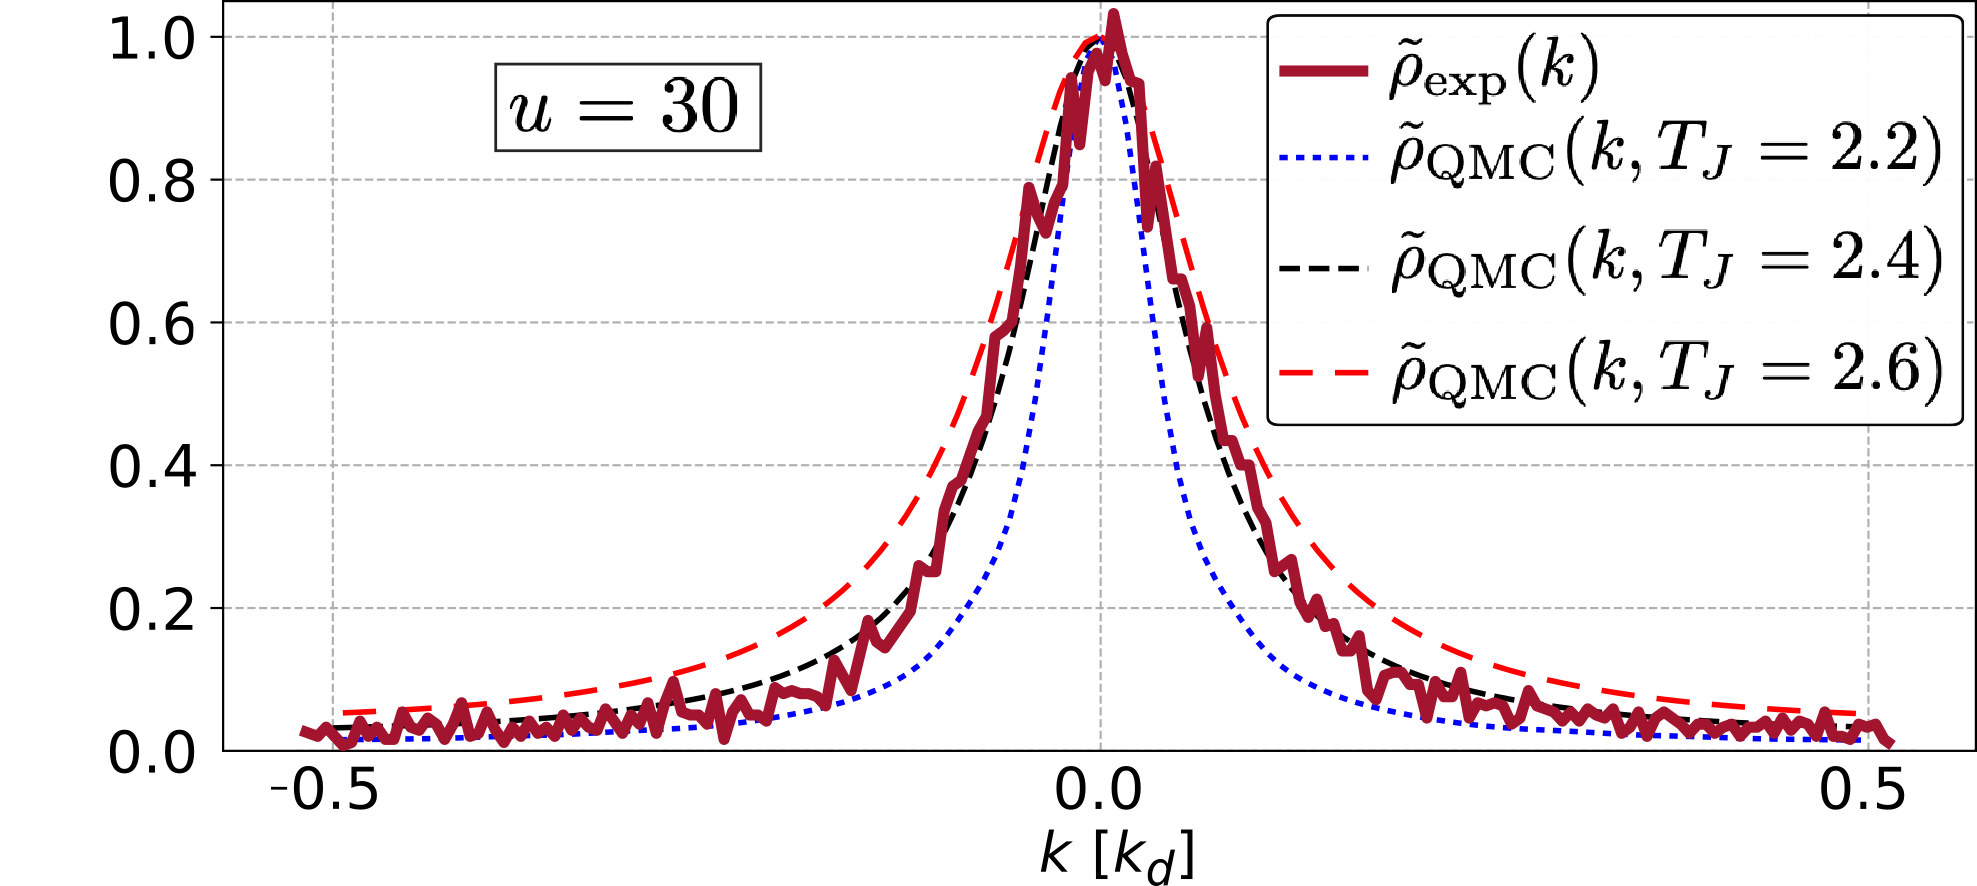
\includegraphics[width=0.8\textwidth]{Fig/Chapter3/comp_qmc.png}
    \caption{Comparison of experimental and QMC normalized 1D cuts of the momentum density for different temperatures. The ratio $u=30$ corresponds roughly to the location of the critical point in the ground-state.}
    \label{fig:comp_qmc}
\end{figure}

Importantly, these kind of measurements are possible thanks to the 3D single atom resolution of our experimental apparatus. This allows to measure the momentum distribution for low atoms numbers $N \simeq 3,000$ for which QMC calculations are possible down to low temperatures, while providing a great precision on the measurement of $\rho(\bm{k})$ without any line-of-sight integration contrary to optical imaging.

We show on Fig.-\ref{fig:chi_vs_T} plots of $\chi_{\mathrm{r}}^{2}(T_J)$ as a function of the temperature of the QMC calculations at $u=30$, where $T_J$ is the reduced temperature $T_J = \kB T /J$. We observe a clear minimum that indicates the temperature in the experiment. Interestingly, the close to the minimum value $\chi_{\mathrm{r}}^{2}\left(T_{J}=2.4\right)=3.6 \pm 3.0$ is compatible with unity, meaning that the QMC calculations indeed reproduce the experimental data within the statistical uncertainty. We fit the data with a parabolic profile to identify the position of the minimum. The error on the fit gives us an estimate of the minimal error on the evaluation of the temperature with this technique that can be linked to the notion of Fisher information that we will see in the next paragraph. Note however that in order not to rely on a fit for every data sets, we will estimate the error bars by determining the temperature interval over which distinct values of $\chi_{\mathrm{r}}^{2}$ are observed.

\begin{figure}
    \centering
    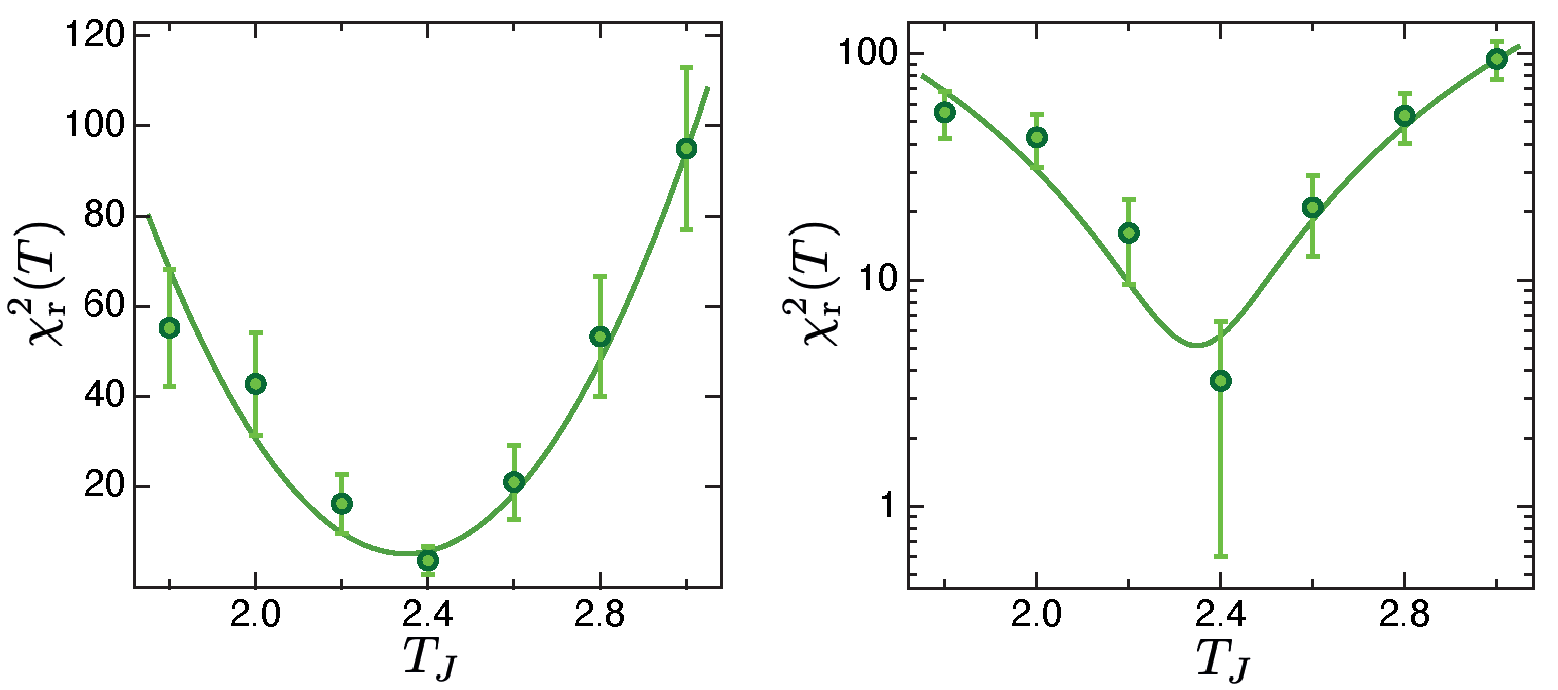
\includegraphics[width=1\textwidth]{Fig/Chapter3/chi_square.pdf}
    \caption{ $\chi_{\mathrm{r}}^{2}(T)$ as a function of temperature in linear and logscale. We clearly identify a minimum from which we deduce the value of $T$ in the experiment.}
    \label{fig:chi_vs_T}
\end{figure}

\subsubsection{Temperature and entropy as a function of $u$}

\begin{figure}
    \centering
    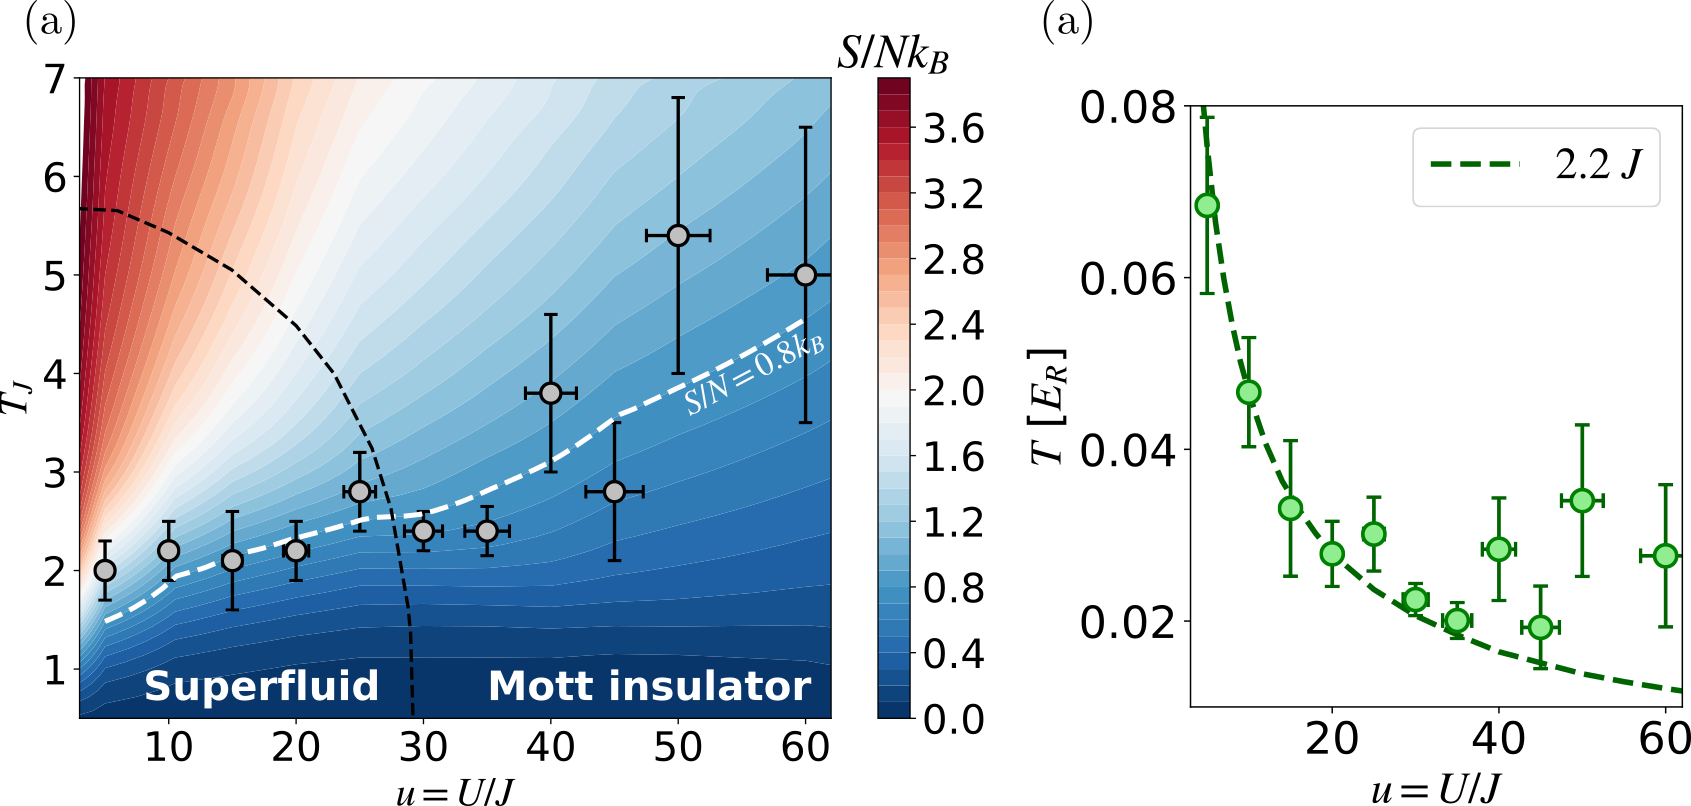
\includegraphics[width=\textwidth]{Fig/Chapter3/temperature.png}
    \caption{(a) Experimental reduced temperature $T_J=\kB T/J$ as a function of $u$. The underlying false color plot shows the theoretical map of the entropy per particle $S/N \kB$ of the trapped 3D Bose-Hubbard model with the experimental parameters. The white dashed line is the isoentropic line $S/N=0.8 \ \kB$. The black dashed line represents the line of critical temperatures for the uniform 3D Bose-Hubbard model at unit lattice filling \cite{capogrosso2007phase}. (b) Absolute temperature in recoil units $E_{\rm{r}}$ as a function of $u$. The green dashed line corresponds to an energy $2.2 J$ (in units of $J$) that best matches the experimental data in the range $u=5-20$.}
    \label{fig:T_vs_u}
\end{figure}

We plot on Fig-\ref{fig:T_vs_u} panel (a) the extracted values of $T_J$ as a function $u$ spanning the phase diagram. The experimental data is plotted alongside to the theoretical map of entropy. Note that we choose to plot the reduced temperature $T_J$ to normalize the adiabatic cooling effect occurring when $u$ increases as illustrated on Fig-\ref{fig:T_vs_u} panel (b). This effect comes from the fact that the isoentropic gas is contained in a Bloch band whose width is proportional to $J$ and decreases with $s$ (see Chapter \ref{sec:chapter_2}). For this reason, the density of states increases with $s$, explaining why $T$ goes down to keep the entropy constant.

The value of the entropy is obtained from the QMC calculations giving the average energy by particle $e(T)$ for various values of the temperature. The energy is then fitted with a high-order polynomial function to compute the specific heat $c(T)=\mathrm{d} e(T) / \mathrm{d} T$ and finally the entropy $S(T) / N=\int_{0}^{T} d \theta c(\theta) / \theta$. The values of the entropy are shown in Fig-\ref{fig:T_vs_u} in false colors. The light white lines represent isoentropic lines. We see that all experimental points are compatible with the isentropic curves spanning the entropy range $S/N= 0.8(1) \ \kB$. These observations are consistent with our assumption that the lattice ramps create a series of thermal equilibrium states that we go through adiabatically conserving the entropy, thus certifying the experimental adiabatic preparation of equilibrium states of the 3D Bose-Hubbard model.

How can we understand the evolution of the isoentropic curve with $u$? For the moderate entropy values of the experiment, we observe to asymptotic regime, the superfluid regime ($u \leq 25$) in which the isoentropic curves grow slowly with $u$, and the Mott insulator regime in which the isoentropic curves grow more rapidly. At low values of $u$, the growth can be understood with Bogoliubov theory. As seen in Chapter \ref{sec:chapter_1}, the speed of sound depends on the strength of the interactions and therefore increases with $u$ $c \propto \sqrt{u}$, decreasing the density of states. The temperature dependence of the entropy is then $\sim T^3/u^2$ so that the isoentropic curves $S/\NBEC \kB =s_0$ should grow as $T \sim s_{0}^{1 / 3} u^{2 / 3}$ (this holds for the homogeneous case and low energies in which the dispersion relation is phononic). On the other hand, in the Mott insulator regime, the entropy writes $S/\NBEC \kB \sim \exp(-\Delta/T)$ where $\Delta \sim u$ is the Mott Insulator gap, giving $T \sim u$ along the isoentropic curves. In addition, we observe a third intermediate regime with a plateau \NOTE{finir ca}


In addition, we measure the entropy per particle in the BEC before loading it into the lattice $S_0/\NBEC \kB$ to see if it matches the entropy measured in the lattice. To evaluate $S_0$, we use the relation for the approximation of a non-interacting, partially-condensed Bose gas in a harmonic trap \cite{pitaevskii2016bose}:

\begin{equation}
    S_{0} / N k_{B}=\frac{4 g_{4}(1)}{\eta(3)}\left(1-f_{c}\right)
\end{equation}

\noindent with $g_{4}(1) \simeq 1.082$, $\eta(3) \simeq 1.2026$ and $f_c$ the condensed fraction.
\NOTE{detailler procédure condensed fraction ?} In the ODT, the thermal energy significantly exceeds the interaction energy, $k_{B} T \sim h \times 2380 \mathrm{~Hz} \gg \mu \sim h \times 350 \mathrm{~Hz}$, meaning that interactions should be negligible, allowing us to use the above equation to find $S_{0} / N= 0.72(7) \ k_{B}$. We compare on Fig.-\ref{fig:entropy_BEC} the measured BEC entropy to the one measured at the various values of $u$ in the lattice. In the region close to $u \simeq 30$ where the error bars are the smallest, we get an excellent agreement, confirming that the loading of the lattice is adiabatic.

\begin{figure}
    \centering
    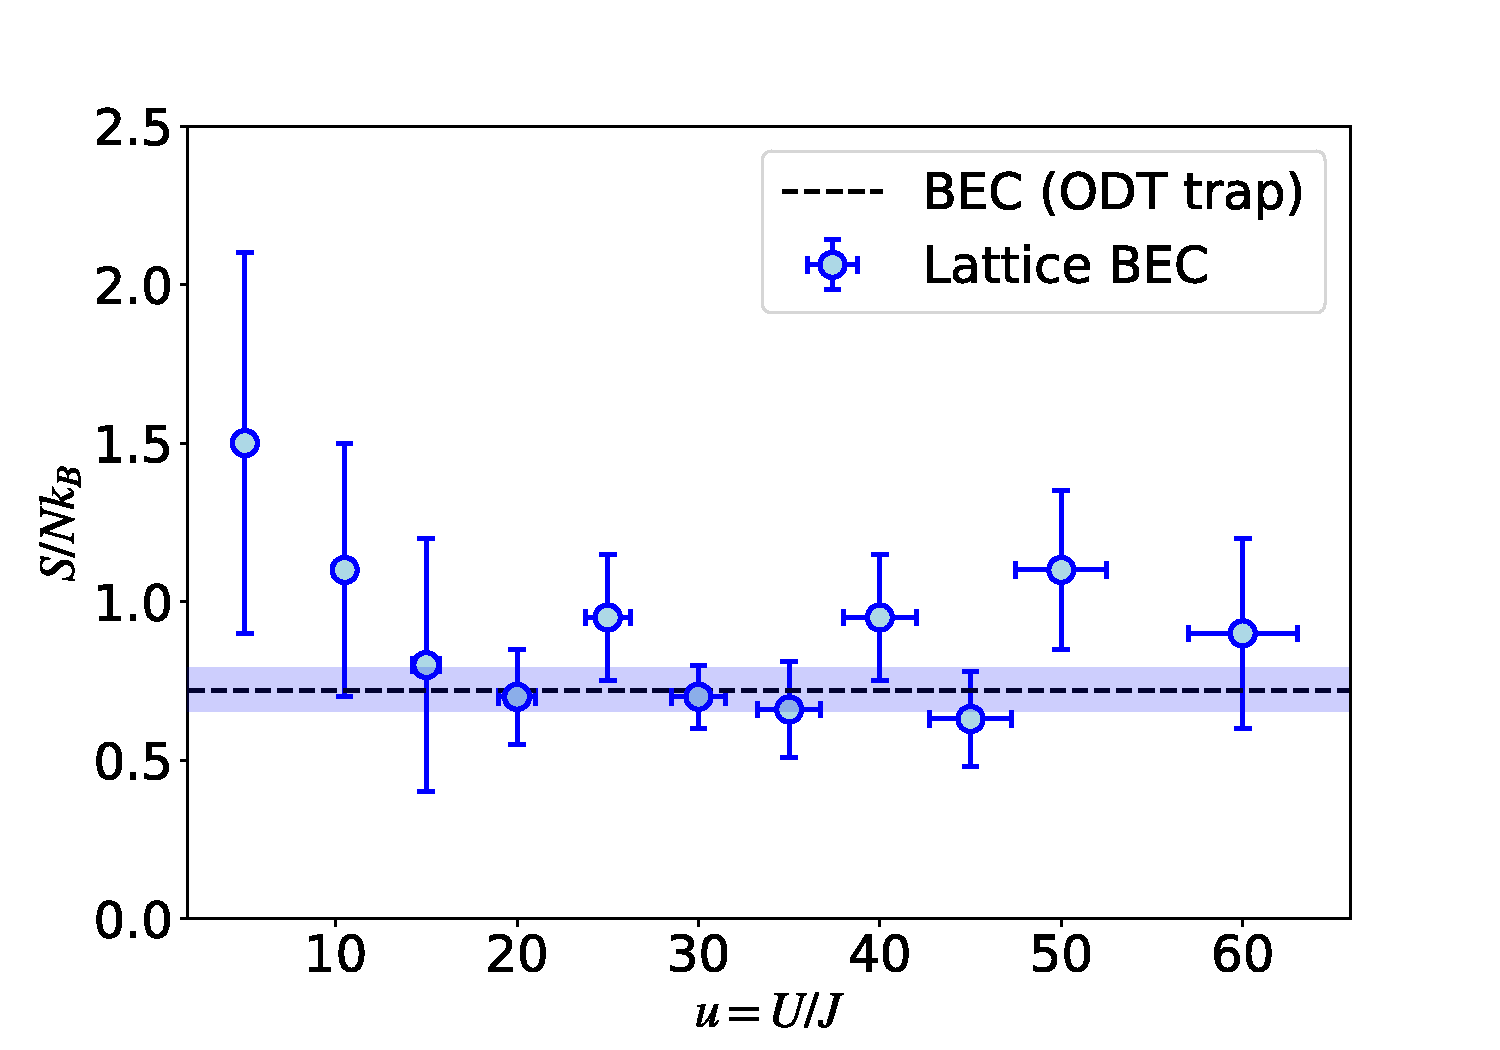
\includegraphics[width=0.8\textwidth]{Fig/Chapter3/entropy_BEC.pdf}
    \caption{Caption}
    \label{fig:entropy_BEC}
\end{figure}

The attentive reader would have noticed on Fig.-\ref{fig:T_vs_u} and Fig.-\ref{fig:comp_qmc} that the vertical error bars on the experimental temperature and entropies vary significantly and are smaller close to the quantum critical point. This effect is described by the Fisher information as we will now see.


\subsection{Fischer information and Cramér-Rao bound}

The concept of \textbf{Fisher information} was introduced by Fisher \cite{fisher1922mathematical} as a mean to quantify the amount of information carried by the distribution of a random variable about a given parameter. In our case, we want to now how well we can determine the parameter temperature by looking at the momentum distribution. The Fisher information writes \cite{van2007parameter}:

\begin{equation}
    I(T)=\sum_{k} \frac{\tilde{\rho}_{\mathrm{QMC}}(k, T)}{\mathcal{N}_{T}}\left[\frac{\partial \log \left(\tilde{\rho}_{\mathrm{QMC}}(k, T) / \mathcal{N}_{T}\right)}{\partial T_{J}}\right]^{2}
\end{equation}



\noindent where $\mathcal{N}_{T}$ is the normalization of $\tilde{\rho}_{\mathrm{QMC}}(k, T)$ summed over all $k$.

The Fisher information tells us what is the minimum uncertainty $\delta T$ with which we can hope to evaluate the temperature through the \textbf{Cramér-Rao} bound that writes:

\begin{equation}
    \delta T_{J}=\frac{k_{B} \delta T}{J} \geq\left(\delta T_{J}\right)_{\min }=\frac{1}{\sqrt{I(T) N_{\rm{runs}}}}
\end{equation}

\noindent Translating the equations into words, the Fisher information tells us how sensitive the momentum density is to variations of the temperature and consequently how precisely we can hope to estimate the temperature by measuring  $\tilde{\rho}_{\mathrm{QMC}}(k, T)$ with finite statistics. We computed the Fisher information across the phase diagram as shown in Fig.-\ref{fig:fisher_info}. We see that the Fisher information varies quite a lot over 4 orders of magnitude. It takes its lower value in the deep Mott region, while it is at its maximum for temperatures where the gas undergoes its transition to a normal gas, consistently with our error bars that we can now compare to the Cramér-Rao bound. We estime that the typical uncertainty on the reduced temperature is $\delta T_J  \sim 0.3$ in the superfluid regime and $\delta T_J  \sim 1.5$ in the deep Mott regime. The former corresponds to $I(T) \sim 1$ and $(\delta T_J)_{\rm{min}} \sim 0.4$ and the latter to  $I(T) \sim 10^{-3}$ and $(\delta T_J)_{\rm{min}} \sim 1.3$. Close to the Mott transition, $I(T) \sim 7$ and $(\delta T_J)_{\rm{min}} \sim 0.02$. With the parabolic fit method of Fig.\ref{fig:chi_vs_T}, we evaluate $(\delta T_J)=0.03$ at $u=30$, thus nearly reaching the Cramér-Rao bound. We are thus always close to saturating the limit set by the Fisher information, meaning that we essentially extract all the possible information on the temperature from the measurement of the momentum density.

\begin{figure}
    \centering
    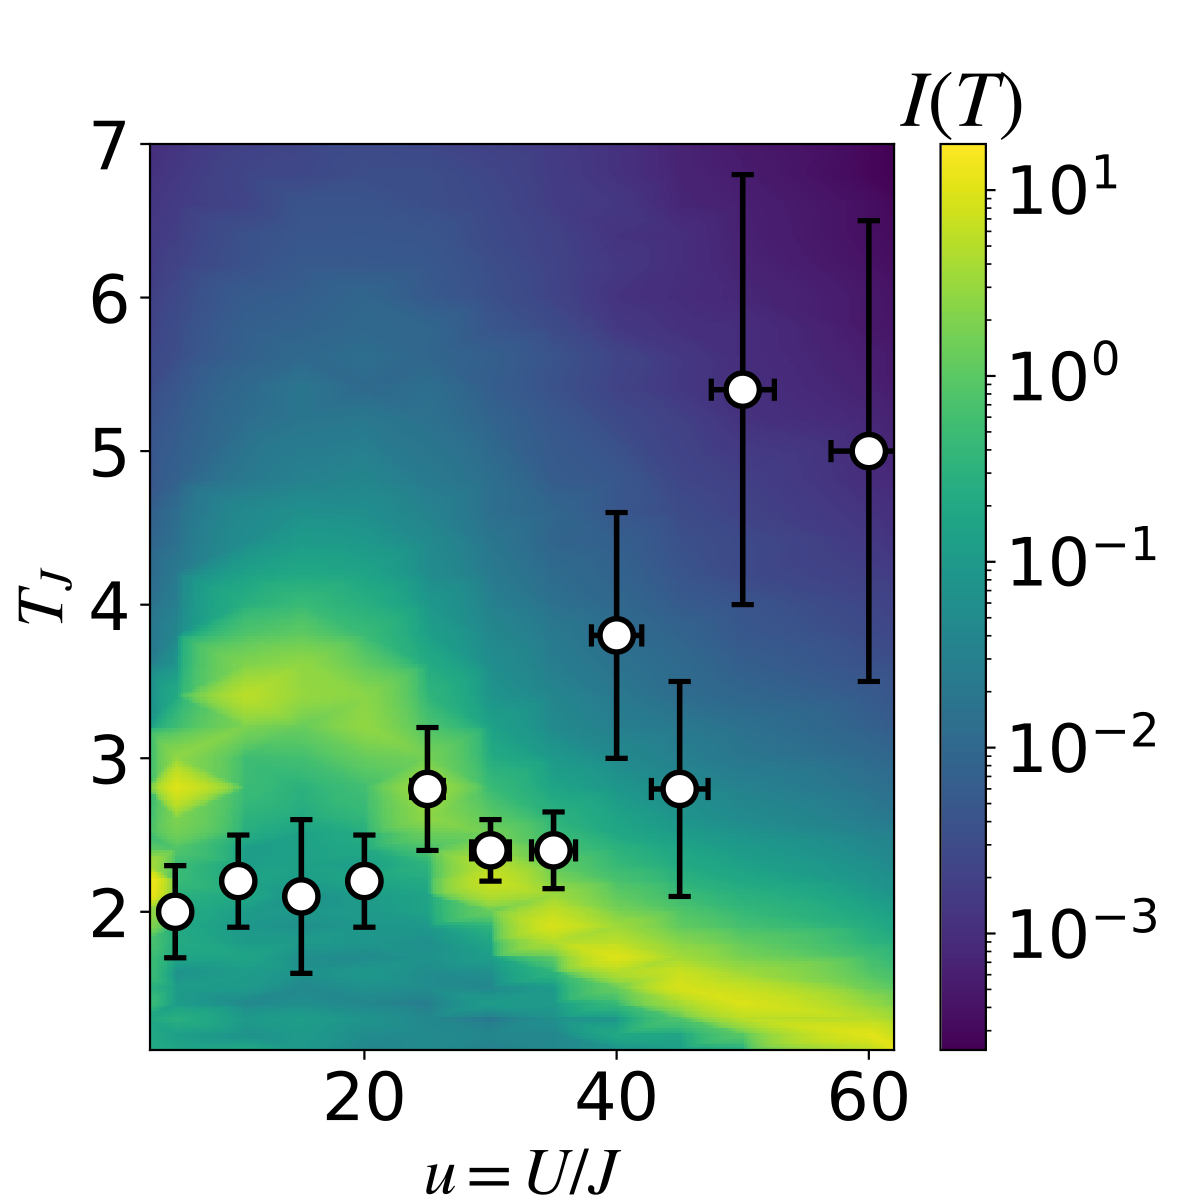
\includegraphics[width=0.7\textwidth]{Fig/Chapter3/fisher_info.png}
    \caption{Caption}
    \label{fig:fisher_info}
\end{figure}


